\documentclass[]{book}
\usepackage{lmodern}
\usepackage{amssymb,amsmath}
\usepackage{ifxetex,ifluatex}
\usepackage{fixltx2e} % provides \textsubscript
\ifnum 0\ifxetex 1\fi\ifluatex 1\fi=0 % if pdftex
  \usepackage[T1]{fontenc}
  \usepackage[utf8]{inputenc}
\else % if luatex or xelatex
  \ifxetex
    \usepackage{mathspec}
  \else
    \usepackage{fontspec}
  \fi
  \defaultfontfeatures{Ligatures=TeX,Scale=MatchLowercase}
\fi
% use upquote if available, for straight quotes in verbatim environments
\IfFileExists{upquote.sty}{\usepackage{upquote}}{}
% use microtype if available
\IfFileExists{microtype.sty}{%
\usepackage{microtype}
\UseMicrotypeSet[protrusion]{basicmath} % disable protrusion for tt fonts
}{}
\usepackage[margin=1in]{geometry}
\usepackage{hyperref}
\hypersetup{unicode=true,
            pdftitle={LDA Tutorial},
            pdfauthor={Chris Tufts},
            pdfborder={0 0 0},
            breaklinks=true}
\urlstyle{same}  % don't use monospace font for urls
\usepackage{color}
\usepackage{fancyvrb}
\newcommand{\VerbBar}{|}
\newcommand{\VERB}{\Verb[commandchars=\\\{\}]}
\DefineVerbatimEnvironment{Highlighting}{Verbatim}{commandchars=\\\{\}}
% Add ',fontsize=\small' for more characters per line
\usepackage{framed}
\definecolor{shadecolor}{RGB}{248,248,248}
\newenvironment{Shaded}{\begin{snugshade}}{\end{snugshade}}
\newcommand{\KeywordTok}[1]{\textcolor[rgb]{0.13,0.29,0.53}{\textbf{#1}}}
\newcommand{\DataTypeTok}[1]{\textcolor[rgb]{0.13,0.29,0.53}{#1}}
\newcommand{\DecValTok}[1]{\textcolor[rgb]{0.00,0.00,0.81}{#1}}
\newcommand{\BaseNTok}[1]{\textcolor[rgb]{0.00,0.00,0.81}{#1}}
\newcommand{\FloatTok}[1]{\textcolor[rgb]{0.00,0.00,0.81}{#1}}
\newcommand{\ConstantTok}[1]{\textcolor[rgb]{0.00,0.00,0.00}{#1}}
\newcommand{\CharTok}[1]{\textcolor[rgb]{0.31,0.60,0.02}{#1}}
\newcommand{\SpecialCharTok}[1]{\textcolor[rgb]{0.00,0.00,0.00}{#1}}
\newcommand{\StringTok}[1]{\textcolor[rgb]{0.31,0.60,0.02}{#1}}
\newcommand{\VerbatimStringTok}[1]{\textcolor[rgb]{0.31,0.60,0.02}{#1}}
\newcommand{\SpecialStringTok}[1]{\textcolor[rgb]{0.31,0.60,0.02}{#1}}
\newcommand{\ImportTok}[1]{#1}
\newcommand{\CommentTok}[1]{\textcolor[rgb]{0.56,0.35,0.01}{\textit{#1}}}
\newcommand{\DocumentationTok}[1]{\textcolor[rgb]{0.56,0.35,0.01}{\textbf{\textit{#1}}}}
\newcommand{\AnnotationTok}[1]{\textcolor[rgb]{0.56,0.35,0.01}{\textbf{\textit{#1}}}}
\newcommand{\CommentVarTok}[1]{\textcolor[rgb]{0.56,0.35,0.01}{\textbf{\textit{#1}}}}
\newcommand{\OtherTok}[1]{\textcolor[rgb]{0.56,0.35,0.01}{#1}}
\newcommand{\FunctionTok}[1]{\textcolor[rgb]{0.00,0.00,0.00}{#1}}
\newcommand{\VariableTok}[1]{\textcolor[rgb]{0.00,0.00,0.00}{#1}}
\newcommand{\ControlFlowTok}[1]{\textcolor[rgb]{0.13,0.29,0.53}{\textbf{#1}}}
\newcommand{\OperatorTok}[1]{\textcolor[rgb]{0.81,0.36,0.00}{\textbf{#1}}}
\newcommand{\BuiltInTok}[1]{#1}
\newcommand{\ExtensionTok}[1]{#1}
\newcommand{\PreprocessorTok}[1]{\textcolor[rgb]{0.56,0.35,0.01}{\textit{#1}}}
\newcommand{\AttributeTok}[1]{\textcolor[rgb]{0.77,0.63,0.00}{#1}}
\newcommand{\RegionMarkerTok}[1]{#1}
\newcommand{\InformationTok}[1]{\textcolor[rgb]{0.56,0.35,0.01}{\textbf{\textit{#1}}}}
\newcommand{\WarningTok}[1]{\textcolor[rgb]{0.56,0.35,0.01}{\textbf{\textit{#1}}}}
\newcommand{\AlertTok}[1]{\textcolor[rgb]{0.94,0.16,0.16}{#1}}
\newcommand{\ErrorTok}[1]{\textcolor[rgb]{0.64,0.00,0.00}{\textbf{#1}}}
\newcommand{\NormalTok}[1]{#1}
\usepackage{longtable,booktabs}
\usepackage{graphicx,grffile}
\makeatletter
\def\maxwidth{\ifdim\Gin@nat@width>\linewidth\linewidth\else\Gin@nat@width\fi}
\def\maxheight{\ifdim\Gin@nat@height>\textheight\textheight\else\Gin@nat@height\fi}
\makeatother
% Scale images if necessary, so that they will not overflow the page
% margins by default, and it is still possible to overwrite the defaults
% using explicit options in \includegraphics[width, height, ...]{}
\setkeys{Gin}{width=\maxwidth,height=\maxheight,keepaspectratio}
\IfFileExists{parskip.sty}{%
\usepackage{parskip}
}{% else
\setlength{\parindent}{0pt}
\setlength{\parskip}{6pt plus 2pt minus 1pt}
}
\setlength{\emergencystretch}{3em}  % prevent overfull lines
\providecommand{\tightlist}{%
  \setlength{\itemsep}{0pt}\setlength{\parskip}{0pt}}
\setcounter{secnumdepth}{5}
% Redefines (sub)paragraphs to behave more like sections
\ifx\paragraph\undefined\else
\let\oldparagraph\paragraph
\renewcommand{\paragraph}[1]{\oldparagraph{#1}\mbox{}}
\fi
\ifx\subparagraph\undefined\else
\let\oldsubparagraph\subparagraph
\renewcommand{\subparagraph}[1]{\oldsubparagraph{#1}\mbox{}}
\fi

%%% Use protect on footnotes to avoid problems with footnotes in titles
\let\rmarkdownfootnote\footnote%
\def\footnote{\protect\rmarkdownfootnote}

%%% Change title format to be more compact
\usepackage{titling}

% Create subtitle command for use in maketitle
\newcommand{\subtitle}[1]{
  \posttitle{
    \begin{center}\large#1\end{center}
    }
}

\setlength{\droptitle}{-2em}
  \title{LDA Tutorial}
  \pretitle{\vspace{\droptitle}\centering\huge}
  \posttitle{\par}
  \author{Chris Tufts}
  \preauthor{\centering\large\emph}
  \postauthor{\par}
  \date{}
  \predate{}\postdate{}


\usepackage{amsthm}
\newtheorem{theorem}{Theorem}[chapter]
\newtheorem{lemma}{Lemma}[chapter]
\theoremstyle{definition}
\newtheorem{definition}{Definition}[chapter]
\newtheorem{corollary}{Corollary}[chapter]
\newtheorem{proposition}{Proposition}[chapter]
\theoremstyle{definition}
\newtheorem{example}{Example}[chapter]
\theoremstyle{definition}
\newtheorem{exercise}{Exercise}[chapter]
\theoremstyle{remark}
\newtheorem*{remark}{Remark}
\newtheorem*{solution}{Solution}
\begin{document}
\maketitle

{
\setcounter{tocdepth}{1}
\tableofcontents
}
\chapter*{Preface}\label{preface}
\addcontentsline{toc}{chapter}{Preface}

\chapter{What is LDA?}\label{what-is-lda}

\section{Animal Generator}\label{animal-generator}

\section{Inference}\label{inference}

Inference

\chapter{Parameter Estimation}\label{parameter-estimation}

LDA is a generative probabilistic model, so to understand exactly how
this works we need to understand the underlying probability
distibutions. In this chapter we will focus on the Bernoulli
distribution and the Beta distribution. Both of these distributions are
very closely related to (and also special cases of) the multinomial and
Dirichlet distributions utilized by LDA, but they are a bit easier to
comprehend. Once we have made our way through Bernoulli and beta, the
following chapter will go into detail about multinomial and Dirichlet
distributions and how all these peices are connected.

Throughout the chapter I'm going to build off of a simple example - a
single coin flip. Let's begin.

\section{Distributions}\label{distributions}

\subsection{Bernoulli}\label{bernoulli}

When you flip a coin you get either heads or tails as an outcome
(barring the possibility it lands on it's side). This single coin flip
is an example of a Bernoulli trial and we can use the Bernoulli
distribution to calculate the probability of either outcome. Any single
trial with two possible outcomes can be modeled as a Bernoulli trial:
team wins/loses, pitch is a strike/ball, coin comes up heads or tails,
etc.

\subsubsection{Bernoulli: A Special Case of the Binomial
Distribution}\label{bernoulli-a-special-case-of-the-binomial-distribution}

You will often see Bernoulli distribution mentioned as a special case of
the Binomial distribution. The binomial model consists of \emph{n}
Bernoulli trials, where each trial is independent and the probability of
success does not change between trials.(Kerns
\protect\hyperlink{ref-kerns2010introduction}{2010}). The Bernoulli
distribution is the case of a single trial or \emph{n}=1.

\textbf{NOTE:} I will use the term success interchangably with the term
heads when describing bernoulli distribution. In reality success could
be tails if you choose to define it that way.

To clarify, if I want to calculate the probability of getting heads on a
single coin flip I will use a bernoulli distribution. However, if I want
to know the probability of getting 2 heads (or more) in a row, this is
where the binomial distribution comes in. For our purposes we are only
concerned about the outcome of a single coin flip and will therefore
stick to the Bernoulli distribution.

\begin{figure}
\centering
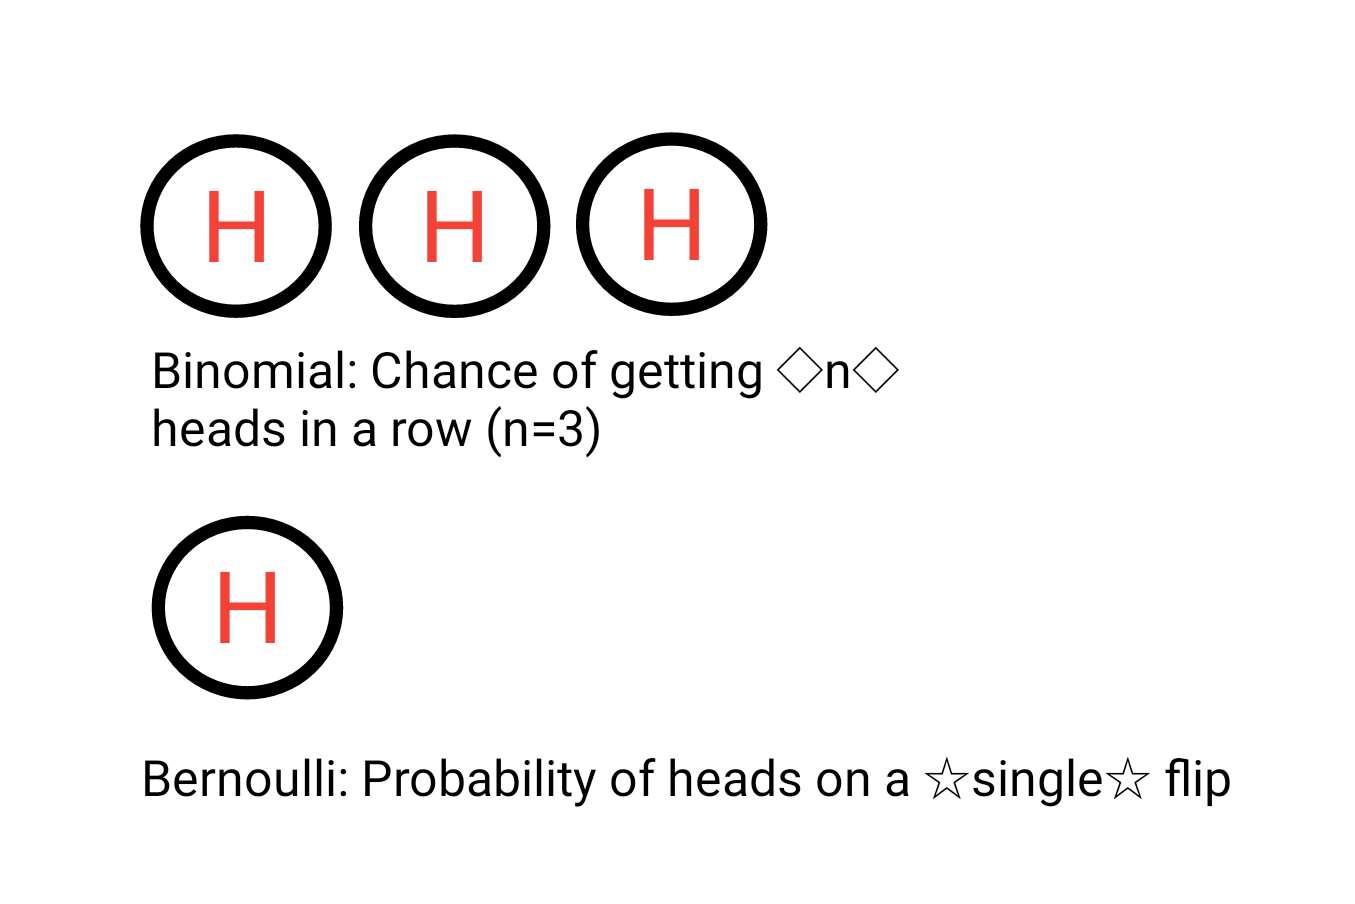
\includegraphics{Images/Bern_Binomial.png}
\caption{\label{fig:BernVSBin}Bernoulli and Binomial Distributions}
\end{figure}

\subsubsection{Bernoulli - Distribution
Notation}\label{bernoulli---distribution-notation}

The probability mass function of the bernoulli distribution is shown in
Equation 1.

\[
f_{x}(x)=P(X=x)=\theta^{x}(1-\theta)^{1-x}, \hspace{1cm} x = \{0,1\} 
\tag{1}
\]

The only parameter of the bernoulli distribution is \(\theta\), which
defines the probability of success during a bernoulli trial. The value
of \emph{x} is 0 for a failure and 1 for a success. In a practical
example you can think of this as 0 for tails and 1 for heads during a
coin flip. In Equation 2 the value of \(\theta\) is set to 0.7. We can
see the probability of getting a success is 0.7, while the probability
of failure is 0.3.

\[
\begin{aligned}
P(X=1)&=\theta^{1}(1-\theta)^{1-1}, \hspace{1cm} \theta=0.7 \\
P(X=1)&=0.7*1=0.7 \\\\
P(X=0)&=0.7^{0}(1-0.7)^{1-0}\\
P(X=0)&=0.3
\end{aligned}
\tag{2}
\]

\subsection{Beta Distribution}\label{beta-distribution}

The beta distribution can be thought of as a probability distribution of
distributions(Robinson \protect\hyperlink{ref-Robinson2014beta}{2014}).

We know the bernoulli distribution has one parameter, \(\theta\). We can
use the beta distribution to determine the probability of a specific
value of \(\theta\) based on prior information, in our case previous
coin flips.

If you flip a coin 2 times resulting in 1 heads and 1 tails how sure are
you that the coin is fair? Probably not all that sure, right? But what
if you flipped the coin 200 times and it resulted in 100 heads and 100
tails? You would be much more confident that the coin is fair. This is
the basis of the beta distribution.

The beta distribution has 2 shape parameters, \(\alpha\) and \(\beta\).
These can be though of as the results from the coin flips we just talked
about. Below the probability density for different values of \(\theta\)
is displayed based on different values of \(\alpha\) and \(\beta\). In
general, the higher the value of \(\alpha\) and \(\beta\) the narrower
the density curve is. This makes sense with our thought example above,
the more information (\emph{coin flip results}) we have, the more
confident we are in our coin's bias (i.e.~is it fair, head heavy, etc.).

\begin{Shaded}
\begin{Highlighting}[]
\KeywordTok{library}\NormalTok{(tidyverse)}
\end{Highlighting}
\end{Shaded}

\begin{verbatim}
## Loading tidyverse: ggplot2
## Loading tidyverse: tibble
## Loading tidyverse: tidyr
## Loading tidyverse: readr
## Loading tidyverse: purrr
## Loading tidyverse: dplyr
\end{verbatim}

\begin{verbatim}
## Warning: package 'tidyr' was built under R version 3.4.2
\end{verbatim}

\begin{verbatim}
## Warning: package 'purrr' was built under R version 3.4.2
\end{verbatim}

\begin{verbatim}
## Warning: package 'dplyr' was built under R version 3.4.2
\end{verbatim}

\begin{verbatim}
## Conflicts with tidy packages ----------------------------------------------
\end{verbatim}

\begin{verbatim}
## filter(): dplyr, stats
## lag():    dplyr, stats
\end{verbatim}

\begin{Shaded}
\begin{Highlighting}[]
\NormalTok{a <-}\StringTok{ }\KeywordTok{c}\NormalTok{(}\DecValTok{1}\NormalTok{, }\DecValTok{10}\NormalTok{, }\DecValTok{100}\NormalTok{)}
\NormalTok{b <-}\StringTok{ }\KeywordTok{c}\NormalTok{(}\DecValTok{1}\NormalTok{, }\DecValTok{10}\NormalTok{, }\DecValTok{100}\NormalTok{)}
\NormalTok{params <-}\StringTok{ }\KeywordTok{cbind}\NormalTok{(a,b)}
\NormalTok{ds <-}\StringTok{ }\OtherTok{NULL}
\NormalTok{n <-}\StringTok{ }\KeywordTok{seq}\NormalTok{(}\DecValTok{0}\NormalTok{,}\DecValTok{1}\NormalTok{,}\FloatTok{0.01}\NormalTok{)}
\ControlFlowTok{for}\NormalTok{(i }\ControlFlowTok{in} \DecValTok{1}\OperatorTok{:}\KeywordTok{nrow}\NormalTok{(params))\{}
\NormalTok{  ds <-}\StringTok{ }\KeywordTok{rbind}\NormalTok{(}\KeywordTok{data.frame}\NormalTok{(}\DataTypeTok{x =}\NormalTok{ n, }\DataTypeTok{y =} \KeywordTok{dbeta}\NormalTok{(n, params[i,}\DecValTok{1}\NormalTok{], params[i,}\DecValTok{2}\NormalTok{]),}
                             \DataTypeTok{parameters =} \KeywordTok{paste0}\NormalTok{(}\StringTok{"\textbackslash{}U03B1 = "}\NormalTok{,params[i,}\DecValTok{1}\NormalTok{],}
                                                 \StringTok{", \textbackslash{}U03B2 = "}\NormalTok{, params[i,}\DecValTok{2}\NormalTok{])), ds)}
\NormalTok{\}}

\KeywordTok{ggplot}\NormalTok{(ds, }\KeywordTok{aes}\NormalTok{(}\DataTypeTok{x =}\NormalTok{ x, }\DataTypeTok{y =}\NormalTok{ y, }\DataTypeTok{color=}\NormalTok{parameters)) }\OperatorTok{+}\StringTok{ }\KeywordTok{geom_line}\NormalTok{() }\OperatorTok{+}\StringTok{ }
\StringTok{  }\KeywordTok{labs}\NormalTok{(}\DataTypeTok{x =} \StringTok{'\textbackslash{}U03B8'}\NormalTok{, }\DataTypeTok{y =} \StringTok{'Probability Density'}\NormalTok{) }\OperatorTok{+}
\StringTok{  }\KeywordTok{scale_color_discrete}\NormalTok{(}\DataTypeTok{name=}\OtherTok{NULL}\NormalTok{) }\OperatorTok{+}\StringTok{ }\KeywordTok{theme_minimal}\NormalTok{()}
\end{Highlighting}
\end{Shaded}

\begin{verbatim}
## Warning in grid.Call(C_stringMetric, as.graphicsAnnot(x$label)): font
## metrics unknown for Unicode character U+03b8
\end{verbatim}

\begin{verbatim}
## Warning in grid.Call(C_stringMetric, as.graphicsAnnot(x$label)): font
## metrics unknown for Unicode character U+03b8
\end{verbatim}

\begin{verbatim}
## Warning in grid.Call(C_stringMetric, as.graphicsAnnot(x$label)): conversion
## failure on 'θ' in 'mbcsToSbcs': dot substituted for <ce>
\end{verbatim}

\begin{verbatim}
## Warning in grid.Call(C_stringMetric, as.graphicsAnnot(x$label)): conversion
## failure on 'θ' in 'mbcsToSbcs': dot substituted for <b8>
\end{verbatim}

\begin{verbatim}
## Warning in grid.Call(C_stringMetric, as.graphicsAnnot(x$label)): font
## metrics unknown for Unicode character U+03b1
\end{verbatim}

\begin{verbatim}
## Warning in grid.Call(C_stringMetric, as.graphicsAnnot(x$label)): font
## metrics unknown for Unicode character U+03b2
\end{verbatim}

\begin{verbatim}
## Warning in grid.Call(C_stringMetric, as.graphicsAnnot(x$label)): font
## metrics unknown for Unicode character U+03b1
\end{verbatim}

\begin{verbatim}
## Warning in grid.Call(C_stringMetric, as.graphicsAnnot(x$label)): font
## metrics unknown for Unicode character U+03b2
\end{verbatim}

\begin{verbatim}
## Warning in grid.Call(C_stringMetric, as.graphicsAnnot(x$label)): conversion
## failure on 'α = 100, β = 100' in 'mbcsToSbcs': dot substituted for <ce>
\end{verbatim}

\begin{verbatim}
## Warning in grid.Call(C_stringMetric, as.graphicsAnnot(x$label)): conversion
## failure on 'α = 100, β = 100' in 'mbcsToSbcs': dot substituted for <b1>
\end{verbatim}

\begin{verbatim}
## Warning in grid.Call(C_stringMetric, as.graphicsAnnot(x$label)): conversion
## failure on 'α = 100, β = 100' in 'mbcsToSbcs': dot substituted for <ce>
\end{verbatim}

\begin{verbatim}
## Warning in grid.Call(C_stringMetric, as.graphicsAnnot(x$label)): conversion
## failure on 'α = 100, β = 100' in 'mbcsToSbcs': dot substituted for <b2>
\end{verbatim}

\begin{verbatim}
## Warning in grid.Call(C_stringMetric, as.graphicsAnnot(x$label)): font
## metrics unknown for Unicode character U+03b1
\end{verbatim}

\begin{verbatim}
## Warning in grid.Call(C_stringMetric, as.graphicsAnnot(x$label)): font
## metrics unknown for Unicode character U+03b2
\end{verbatim}

\begin{verbatim}
## Warning in grid.Call(C_stringMetric, as.graphicsAnnot(x$label)): font
## metrics unknown for Unicode character U+03b1
\end{verbatim}

\begin{verbatim}
## Warning in grid.Call(C_stringMetric, as.graphicsAnnot(x$label)): font
## metrics unknown for Unicode character U+03b2
\end{verbatim}

\begin{verbatim}
## Warning in grid.Call(C_stringMetric, as.graphicsAnnot(x$label)): conversion
## failure on 'α = 10, β = 10' in 'mbcsToSbcs': dot substituted for <ce>
\end{verbatim}

\begin{verbatim}
## Warning in grid.Call(C_stringMetric, as.graphicsAnnot(x$label)): conversion
## failure on 'α = 10, β = 10' in 'mbcsToSbcs': dot substituted for <b1>
\end{verbatim}

\begin{verbatim}
## Warning in grid.Call(C_stringMetric, as.graphicsAnnot(x$label)): conversion
## failure on 'α = 10, β = 10' in 'mbcsToSbcs': dot substituted for <ce>
\end{verbatim}

\begin{verbatim}
## Warning in grid.Call(C_stringMetric, as.graphicsAnnot(x$label)): conversion
## failure on 'α = 10, β = 10' in 'mbcsToSbcs': dot substituted for <b2>
\end{verbatim}

\begin{verbatim}
## Warning in grid.Call(C_stringMetric, as.graphicsAnnot(x$label)): font
## metrics unknown for Unicode character U+03b1
\end{verbatim}

\begin{verbatim}
## Warning in grid.Call(C_stringMetric, as.graphicsAnnot(x$label)): font
## metrics unknown for Unicode character U+03b2
\end{verbatim}

\begin{verbatim}
## Warning in grid.Call(C_stringMetric, as.graphicsAnnot(x$label)): font
## metrics unknown for Unicode character U+03b1
\end{verbatim}

\begin{verbatim}
## Warning in grid.Call(C_stringMetric, as.graphicsAnnot(x$label)): font
## metrics unknown for Unicode character U+03b2
\end{verbatim}

\begin{verbatim}
## Warning in grid.Call(C_stringMetric, as.graphicsAnnot(x$label)): conversion
## failure on 'α = 1, β = 1' in 'mbcsToSbcs': dot substituted for <ce>
\end{verbatim}

\begin{verbatim}
## Warning in grid.Call(C_stringMetric, as.graphicsAnnot(x$label)): conversion
## failure on 'α = 1, β = 1' in 'mbcsToSbcs': dot substituted for <b1>
\end{verbatim}

\begin{verbatim}
## Warning in grid.Call(C_stringMetric, as.graphicsAnnot(x$label)): conversion
## failure on 'α = 1, β = 1' in 'mbcsToSbcs': dot substituted for <ce>
\end{verbatim}

\begin{verbatim}
## Warning in grid.Call(C_stringMetric, as.graphicsAnnot(x$label)): conversion
## failure on 'α = 1, β = 1' in 'mbcsToSbcs': dot substituted for <b2>
\end{verbatim}

\begin{verbatim}
## Warning in grid.Call(C_textBounds, as.graphicsAnnot(x$label), x$x, x$y, :
## conversion failure on 'α = 100, β = 100' in 'mbcsToSbcs': dot substituted
## for <ce>
\end{verbatim}

\begin{verbatim}
## Warning in grid.Call(C_textBounds, as.graphicsAnnot(x$label), x$x, x$y, :
## conversion failure on 'α = 100, β = 100' in 'mbcsToSbcs': dot substituted
## for <b1>
\end{verbatim}

\begin{verbatim}
## Warning in grid.Call(C_textBounds, as.graphicsAnnot(x$label), x$x, x$y, :
## conversion failure on 'α = 100, β = 100' in 'mbcsToSbcs': dot substituted
## for <ce>
\end{verbatim}

\begin{verbatim}
## Warning in grid.Call(C_textBounds, as.graphicsAnnot(x$label), x$x, x$y, :
## conversion failure on 'α = 100, β = 100' in 'mbcsToSbcs': dot substituted
## for <b2>
\end{verbatim}

\begin{verbatim}
## Warning in grid.Call(C_textBounds, as.graphicsAnnot(x$label), x$x, x$y, :
## conversion failure on 'α = 100, β = 100' in 'mbcsToSbcs': dot substituted
## for <ce>
\end{verbatim}

\begin{verbatim}
## Warning in grid.Call(C_textBounds, as.graphicsAnnot(x$label), x$x, x$y, :
## conversion failure on 'α = 100, β = 100' in 'mbcsToSbcs': dot substituted
## for <b1>
\end{verbatim}

\begin{verbatim}
## Warning in grid.Call(C_textBounds, as.graphicsAnnot(x$label), x$x, x$y, :
## conversion failure on 'α = 100, β = 100' in 'mbcsToSbcs': dot substituted
## for <ce>
\end{verbatim}

\begin{verbatim}
## Warning in grid.Call(C_textBounds, as.graphicsAnnot(x$label), x$x, x$y, :
## conversion failure on 'α = 100, β = 100' in 'mbcsToSbcs': dot substituted
## for <b2>
\end{verbatim}

\begin{verbatim}
## Warning in grid.Call(C_textBounds, as.graphicsAnnot(x$label), x$x, x$y, :
## conversion failure on 'α = 10, β = 10' in 'mbcsToSbcs': dot substituted for
## <ce>
\end{verbatim}

\begin{verbatim}
## Warning in grid.Call(C_textBounds, as.graphicsAnnot(x$label), x$x, x$y, :
## conversion failure on 'α = 10, β = 10' in 'mbcsToSbcs': dot substituted for
## <b1>
\end{verbatim}

\begin{verbatim}
## Warning in grid.Call(C_textBounds, as.graphicsAnnot(x$label), x$x, x$y, :
## conversion failure on 'α = 10, β = 10' in 'mbcsToSbcs': dot substituted for
## <ce>
\end{verbatim}

\begin{verbatim}
## Warning in grid.Call(C_textBounds, as.graphicsAnnot(x$label), x$x, x$y, :
## conversion failure on 'α = 10, β = 10' in 'mbcsToSbcs': dot substituted for
## <b2>
\end{verbatim}

\begin{verbatim}
## Warning in grid.Call(C_textBounds, as.graphicsAnnot(x$label), x$x, x$y, :
## conversion failure on 'α = 10, β = 10' in 'mbcsToSbcs': dot substituted for
## <ce>
\end{verbatim}

\begin{verbatim}
## Warning in grid.Call(C_textBounds, as.graphicsAnnot(x$label), x$x, x$y, :
## conversion failure on 'α = 10, β = 10' in 'mbcsToSbcs': dot substituted for
## <b1>
\end{verbatim}

\begin{verbatim}
## Warning in grid.Call(C_textBounds, as.graphicsAnnot(x$label), x$x, x$y, :
## conversion failure on 'α = 10, β = 10' in 'mbcsToSbcs': dot substituted for
## <ce>
\end{verbatim}

\begin{verbatim}
## Warning in grid.Call(C_textBounds, as.graphicsAnnot(x$label), x$x, x$y, :
## conversion failure on 'α = 10, β = 10' in 'mbcsToSbcs': dot substituted for
## <b2>
\end{verbatim}

\begin{verbatim}
## Warning in grid.Call(C_textBounds, as.graphicsAnnot(x$label), x$x, x$y, :
## conversion failure on 'α = 1, β = 1' in 'mbcsToSbcs': dot substituted for
## <ce>
\end{verbatim}

\begin{verbatim}
## Warning in grid.Call(C_textBounds, as.graphicsAnnot(x$label), x$x, x$y, :
## conversion failure on 'α = 1, β = 1' in 'mbcsToSbcs': dot substituted for
## <b1>
\end{verbatim}

\begin{verbatim}
## Warning in grid.Call(C_textBounds, as.graphicsAnnot(x$label), x$x, x$y, :
## conversion failure on 'α = 1, β = 1' in 'mbcsToSbcs': dot substituted for
## <ce>
\end{verbatim}

\begin{verbatim}
## Warning in grid.Call(C_textBounds, as.graphicsAnnot(x$label), x$x, x$y, :
## conversion failure on 'α = 1, β = 1' in 'mbcsToSbcs': dot substituted for
## <b2>
\end{verbatim}

\begin{verbatim}
## Warning in grid.Call(C_textBounds, as.graphicsAnnot(x$label), x$x, x$y, :
## conversion failure on 'α = 1, β = 1' in 'mbcsToSbcs': dot substituted for
## <ce>
\end{verbatim}

\begin{verbatim}
## Warning in grid.Call(C_textBounds, as.graphicsAnnot(x$label), x$x, x$y, :
## conversion failure on 'α = 1, β = 1' in 'mbcsToSbcs': dot substituted for
## <b1>
\end{verbatim}

\begin{verbatim}
## Warning in grid.Call(C_textBounds, as.graphicsAnnot(x$label), x$x, x$y, :
## conversion failure on 'α = 1, β = 1' in 'mbcsToSbcs': dot substituted for
## <ce>
\end{verbatim}

\begin{verbatim}
## Warning in grid.Call(C_textBounds, as.graphicsAnnot(x$label), x$x, x$y, :
## conversion failure on 'α = 1, β = 1' in 'mbcsToSbcs': dot substituted for
## <b2>
\end{verbatim}

\begin{verbatim}
## Warning in grid.Call(C_textBounds, as.graphicsAnnot(x$label), x$x, x$y, :
## conversion failure on 'α = 100, β = 100' in 'mbcsToSbcs': dot substituted
## for <ce>
\end{verbatim}

\begin{verbatim}
## Warning in grid.Call(C_textBounds, as.graphicsAnnot(x$label), x$x, x$y, :
## conversion failure on 'α = 100, β = 100' in 'mbcsToSbcs': dot substituted
## for <b1>
\end{verbatim}

\begin{verbatim}
## Warning in grid.Call(C_textBounds, as.graphicsAnnot(x$label), x$x, x$y, :
## conversion failure on 'α = 100, β = 100' in 'mbcsToSbcs': dot substituted
## for <ce>
\end{verbatim}

\begin{verbatim}
## Warning in grid.Call(C_textBounds, as.graphicsAnnot(x$label), x$x, x$y, :
## conversion failure on 'α = 100, β = 100' in 'mbcsToSbcs': dot substituted
## for <b2>
\end{verbatim}

\begin{verbatim}
## Warning in grid.Call(C_textBounds, as.graphicsAnnot(x$label), x$x, x$y, :
## conversion failure on 'α = 100, β = 100' in 'mbcsToSbcs': dot substituted
## for <ce>
\end{verbatim}

\begin{verbatim}
## Warning in grid.Call(C_textBounds, as.graphicsAnnot(x$label), x$x, x$y, :
## conversion failure on 'α = 100, β = 100' in 'mbcsToSbcs': dot substituted
## for <b1>
\end{verbatim}

\begin{verbatim}
## Warning in grid.Call(C_textBounds, as.graphicsAnnot(x$label), x$x, x$y, :
## conversion failure on 'α = 100, β = 100' in 'mbcsToSbcs': dot substituted
## for <ce>
\end{verbatim}

\begin{verbatim}
## Warning in grid.Call(C_textBounds, as.graphicsAnnot(x$label), x$x, x$y, :
## conversion failure on 'α = 100, β = 100' in 'mbcsToSbcs': dot substituted
## for <b2>
\end{verbatim}

\begin{verbatim}
## Warning in grid.Call(C_textBounds, as.graphicsAnnot(x$label), x$x, x$y, :
## conversion failure on 'α = 10, β = 10' in 'mbcsToSbcs': dot substituted for
## <ce>
\end{verbatim}

\begin{verbatim}
## Warning in grid.Call(C_textBounds, as.graphicsAnnot(x$label), x$x, x$y, :
## conversion failure on 'α = 10, β = 10' in 'mbcsToSbcs': dot substituted for
## <b1>
\end{verbatim}

\begin{verbatim}
## Warning in grid.Call(C_textBounds, as.graphicsAnnot(x$label), x$x, x$y, :
## conversion failure on 'α = 10, β = 10' in 'mbcsToSbcs': dot substituted for
## <ce>
\end{verbatim}

\begin{verbatim}
## Warning in grid.Call(C_textBounds, as.graphicsAnnot(x$label), x$x, x$y, :
## conversion failure on 'α = 10, β = 10' in 'mbcsToSbcs': dot substituted for
## <b2>
\end{verbatim}

\begin{verbatim}
## Warning in grid.Call(C_textBounds, as.graphicsAnnot(x$label), x$x, x$y, :
## conversion failure on 'α = 10, β = 10' in 'mbcsToSbcs': dot substituted for
## <ce>
\end{verbatim}

\begin{verbatim}
## Warning in grid.Call(C_textBounds, as.graphicsAnnot(x$label), x$x, x$y, :
## conversion failure on 'α = 10, β = 10' in 'mbcsToSbcs': dot substituted for
## <b1>
\end{verbatim}

\begin{verbatim}
## Warning in grid.Call(C_textBounds, as.graphicsAnnot(x$label), x$x, x$y, :
## conversion failure on 'α = 10, β = 10' in 'mbcsToSbcs': dot substituted for
## <ce>
\end{verbatim}

\begin{verbatim}
## Warning in grid.Call(C_textBounds, as.graphicsAnnot(x$label), x$x, x$y, :
## conversion failure on 'α = 10, β = 10' in 'mbcsToSbcs': dot substituted for
## <b2>
\end{verbatim}

\begin{verbatim}
## Warning in grid.Call(C_textBounds, as.graphicsAnnot(x$label), x$x, x$y, :
## conversion failure on 'α = 1, β = 1' in 'mbcsToSbcs': dot substituted for
## <ce>
\end{verbatim}

\begin{verbatim}
## Warning in grid.Call(C_textBounds, as.graphicsAnnot(x$label), x$x, x$y, :
## conversion failure on 'α = 1, β = 1' in 'mbcsToSbcs': dot substituted for
## <b1>
\end{verbatim}

\begin{verbatim}
## Warning in grid.Call(C_textBounds, as.graphicsAnnot(x$label), x$x, x$y, :
## conversion failure on 'α = 1, β = 1' in 'mbcsToSbcs': dot substituted for
## <ce>
\end{verbatim}

\begin{verbatim}
## Warning in grid.Call(C_textBounds, as.graphicsAnnot(x$label), x$x, x$y, :
## conversion failure on 'α = 1, β = 1' in 'mbcsToSbcs': dot substituted for
## <b2>
\end{verbatim}

\begin{verbatim}
## Warning in grid.Call(C_textBounds, as.graphicsAnnot(x$label), x$x, x$y, :
## conversion failure on 'α = 1, β = 1' in 'mbcsToSbcs': dot substituted for
## <ce>
\end{verbatim}

\begin{verbatim}
## Warning in grid.Call(C_textBounds, as.graphicsAnnot(x$label), x$x, x$y, :
## conversion failure on 'α = 1, β = 1' in 'mbcsToSbcs': dot substituted for
## <b1>
\end{verbatim}

\begin{verbatim}
## Warning in grid.Call(C_textBounds, as.graphicsAnnot(x$label), x$x, x$y, :
## conversion failure on 'α = 1, β = 1' in 'mbcsToSbcs': dot substituted for
## <ce>
\end{verbatim}

\begin{verbatim}
## Warning in grid.Call(C_textBounds, as.graphicsAnnot(x$label), x$x, x$y, :
## conversion failure on 'α = 1, β = 1' in 'mbcsToSbcs': dot substituted for
## <b2>
\end{verbatim}

\begin{verbatim}
## Warning in grid.Call(C_textBounds, as.graphicsAnnot(x$label), x$x, x$y, :
## conversion failure on 'θ' in 'mbcsToSbcs': dot substituted for <ce>
\end{verbatim}

\begin{verbatim}
## Warning in grid.Call(C_textBounds, as.graphicsAnnot(x$label), x$x, x$y, :
## conversion failure on 'θ' in 'mbcsToSbcs': dot substituted for <b8>
\end{verbatim}

\begin{verbatim}
## Warning in grid.Call(C_textBounds, as.graphicsAnnot(x$label), x$x, x$y, :
## conversion failure on 'θ' in 'mbcsToSbcs': dot substituted for <ce>
\end{verbatim}

\begin{verbatim}
## Warning in grid.Call(C_textBounds, as.graphicsAnnot(x$label), x$x, x$y, :
## conversion failure on 'θ' in 'mbcsToSbcs': dot substituted for <b8>
\end{verbatim}

\begin{verbatim}
## Warning in grid.Call(C_textBounds, as.graphicsAnnot(x$label), x$x, x$y, :
## conversion failure on 'θ' in 'mbcsToSbcs': dot substituted for <ce>
\end{verbatim}

\begin{verbatim}
## Warning in grid.Call(C_textBounds, as.graphicsAnnot(x$label), x$x, x$y, :
## conversion failure on 'θ' in 'mbcsToSbcs': dot substituted for <b8>
\end{verbatim}

\begin{verbatim}
## Warning in grid.Call(C_textBounds, as.graphicsAnnot(x$label), x$x, x$y, :
## conversion failure on 'θ' in 'mbcsToSbcs': dot substituted for <ce>
\end{verbatim}

\begin{verbatim}
## Warning in grid.Call(C_textBounds, as.graphicsAnnot(x$label), x$x, x$y, :
## conversion failure on 'θ' in 'mbcsToSbcs': dot substituted for <b8>
\end{verbatim}

\begin{verbatim}
## Warning in grid.Call(C_textBounds, as.graphicsAnnot(x$label), x$x, x$y, :
## conversion failure on 'θ' in 'mbcsToSbcs': dot substituted for <ce>
\end{verbatim}

\begin{verbatim}
## Warning in grid.Call(C_textBounds, as.graphicsAnnot(x$label), x$x, x$y, :
## conversion failure on 'θ' in 'mbcsToSbcs': dot substituted for <b8>
\end{verbatim}

\begin{verbatim}
## Warning in grid.Call(C_textBounds, as.graphicsAnnot(x$label), x$x, x$y, :
## conversion failure on 'θ' in 'mbcsToSbcs': dot substituted for <ce>
\end{verbatim}

\begin{verbatim}
## Warning in grid.Call(C_textBounds, as.graphicsAnnot(x$label), x$x, x$y, :
## conversion failure on 'θ' in 'mbcsToSbcs': dot substituted for <b8>
\end{verbatim}

\begin{verbatim}
## Warning in grid.Call(C_textBounds, as.graphicsAnnot(x$label), x$x, x$y, :
## conversion failure on 'θ' in 'mbcsToSbcs': dot substituted for <ce>
\end{verbatim}

\begin{verbatim}
## Warning in grid.Call(C_textBounds, as.graphicsAnnot(x$label), x$x, x$y, :
## conversion failure on 'θ' in 'mbcsToSbcs': dot substituted for <b8>
\end{verbatim}

\begin{verbatim}
## Warning in grid.Call.graphics(C_text, as.graphicsAnnot(x$label), x$x, x
## $y, : conversion failure on 'θ' in 'mbcsToSbcs': dot substituted for <ce>
\end{verbatim}

\begin{verbatim}
## Warning in grid.Call.graphics(C_text, as.graphicsAnnot(x$label), x$x, x
## $y, : conversion failure on 'θ' in 'mbcsToSbcs': dot substituted for <b8>
\end{verbatim}

\begin{verbatim}
## Warning in grid.Call.graphics(C_text, as.graphicsAnnot(x$label), x$x, x
## $y, : conversion failure on 'α = 100, β = 100' in 'mbcsToSbcs': dot
## substituted for <ce>
\end{verbatim}

\begin{verbatim}
## Warning in grid.Call.graphics(C_text, as.graphicsAnnot(x$label), x$x, x
## $y, : conversion failure on 'α = 100, β = 100' in 'mbcsToSbcs': dot
## substituted for <b1>
\end{verbatim}

\begin{verbatim}
## Warning in grid.Call.graphics(C_text, as.graphicsAnnot(x$label), x$x, x
## $y, : conversion failure on 'α = 100, β = 100' in 'mbcsToSbcs': dot
## substituted for <ce>
\end{verbatim}

\begin{verbatim}
## Warning in grid.Call.graphics(C_text, as.graphicsAnnot(x$label), x$x, x
## $y, : conversion failure on 'α = 100, β = 100' in 'mbcsToSbcs': dot
## substituted for <b2>
\end{verbatim}

\begin{verbatim}
## Warning in grid.Call.graphics(C_text, as.graphicsAnnot(x$label), x
## $x, x$y, : conversion failure on 'α = 10, β = 10' in 'mbcsToSbcs': dot
## substituted for <ce>
\end{verbatim}

\begin{verbatim}
## Warning in grid.Call.graphics(C_text, as.graphicsAnnot(x$label), x
## $x, x$y, : conversion failure on 'α = 10, β = 10' in 'mbcsToSbcs': dot
## substituted for <b1>
\end{verbatim}

\begin{verbatim}
## Warning in grid.Call.graphics(C_text, as.graphicsAnnot(x$label), x
## $x, x$y, : conversion failure on 'α = 10, β = 10' in 'mbcsToSbcs': dot
## substituted for <ce>
\end{verbatim}

\begin{verbatim}
## Warning in grid.Call.graphics(C_text, as.graphicsAnnot(x$label), x
## $x, x$y, : conversion failure on 'α = 10, β = 10' in 'mbcsToSbcs': dot
## substituted for <b2>
\end{verbatim}

\begin{verbatim}
## Warning in grid.Call.graphics(C_text, as.graphicsAnnot(x$label), x$x, x
## $y, : conversion failure on 'α = 1, β = 1' in 'mbcsToSbcs': dot substituted
## for <ce>
\end{verbatim}

\begin{verbatim}
## Warning in grid.Call.graphics(C_text, as.graphicsAnnot(x$label), x$x, x
## $y, : conversion failure on 'α = 1, β = 1' in 'mbcsToSbcs': dot substituted
## for <b1>
\end{verbatim}

\begin{verbatim}
## Warning in grid.Call.graphics(C_text, as.graphicsAnnot(x$label), x$x, x
## $y, : conversion failure on 'α = 1, β = 1' in 'mbcsToSbcs': dot substituted
## for <ce>
\end{verbatim}

\begin{verbatim}
## Warning in grid.Call.graphics(C_text, as.graphicsAnnot(x$label), x$x, x
## $y, : conversion failure on 'α = 1, β = 1' in 'mbcsToSbcs': dot substituted
## for <b2>
\end{verbatim}

\begin{figure}
\centering
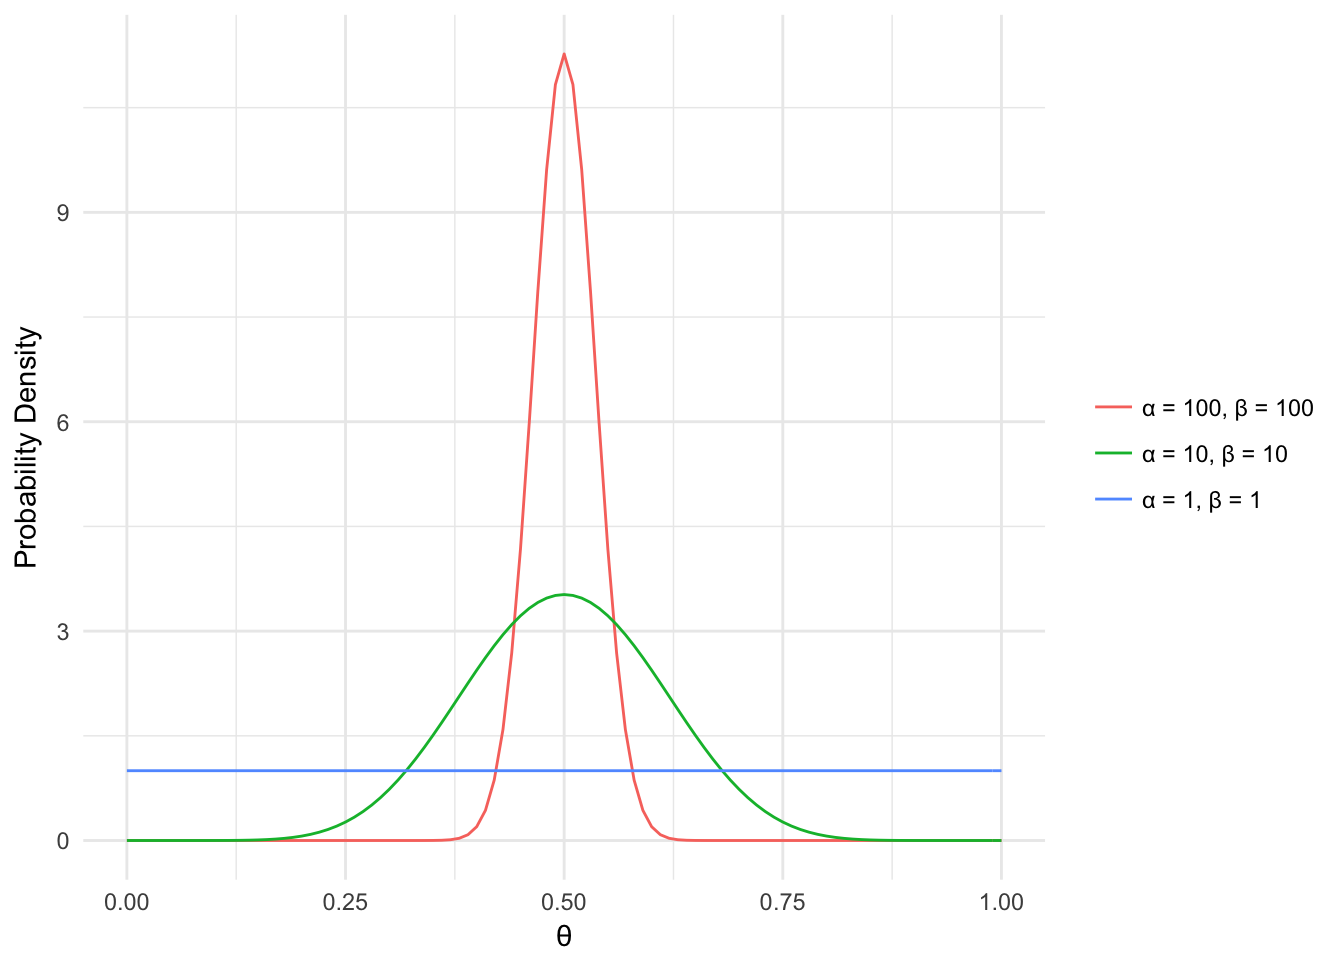
\includegraphics{_main_files/figure-latex/betashape-1.pdf}
\caption{\label{fig:betashape}Beta Distribution}
\end{figure}

What about the cases where \(\alpha\) and \(\beta\) are not equal or
close to equal? Well in those cases you would probably assume a bit of
skew in the distribution, i.e.~your coin may be biased toward head or
tails as shown below.

\begin{Shaded}
\begin{Highlighting}[]
\NormalTok{a <-}\StringTok{ }\KeywordTok{c}\NormalTok{(}\DecValTok{8}\NormalTok{, }\DecValTok{2}\NormalTok{)}
\NormalTok{b <-}\StringTok{ }\KeywordTok{c}\NormalTok{(}\DecValTok{2}\NormalTok{, }\DecValTok{8}\NormalTok{)}
\NormalTok{params <-}\StringTok{ }\KeywordTok{cbind}\NormalTok{(a,b)}
\NormalTok{ds <-}\StringTok{ }\OtherTok{NULL}
\NormalTok{n <-}\StringTok{ }\KeywordTok{seq}\NormalTok{(}\DecValTok{0}\NormalTok{,}\DecValTok{1}\NormalTok{,}\FloatTok{0.01}\NormalTok{)}
\ControlFlowTok{for}\NormalTok{(i }\ControlFlowTok{in} \DecValTok{1}\OperatorTok{:}\KeywordTok{nrow}\NormalTok{(params))\{}
\NormalTok{  ds <-}\StringTok{ }\KeywordTok{rbind}\NormalTok{(}\KeywordTok{data.frame}\NormalTok{(}\DataTypeTok{x =}\NormalTok{ n, }\DataTypeTok{y =} \KeywordTok{dbeta}\NormalTok{(n, params[i,}\DecValTok{1}\NormalTok{], params[i,}\DecValTok{2}\NormalTok{]),}
                             \DataTypeTok{parameters =} \KeywordTok{paste0}\NormalTok{(}\StringTok{"\textbackslash{}U03B1 = "}\NormalTok{,params[i,}\DecValTok{1}\NormalTok{],}
                                                 \StringTok{", \textbackslash{}U03B2 = "}\NormalTok{, params[i,}\DecValTok{2}\NormalTok{])), ds)}
\NormalTok{\}}

\KeywordTok{ggplot}\NormalTok{(ds, }\KeywordTok{aes}\NormalTok{(}\DataTypeTok{x =}\NormalTok{ x, }\DataTypeTok{y =}\NormalTok{ y, }\DataTypeTok{color=}\NormalTok{parameters)) }\OperatorTok{+}\StringTok{ }\KeywordTok{geom_line}\NormalTok{() }\OperatorTok{+}\StringTok{ }
\StringTok{  }\KeywordTok{labs}\NormalTok{(}\DataTypeTok{x =} \StringTok{'\textbackslash{}U03B8'}\NormalTok{, }\DataTypeTok{y =} \StringTok{'Probability Density'}\NormalTok{) }\OperatorTok{+}
\StringTok{  }\KeywordTok{scale_color_manual}\NormalTok{(}\DataTypeTok{name=}\OtherTok{NULL}\NormalTok{, }\DataTypeTok{values =} \KeywordTok{c}\NormalTok{(}\StringTok{"#7A99AC"}\NormalTok{, }\StringTok{"#E4002B"}\NormalTok{)) }\OperatorTok{+}\StringTok{ }\KeywordTok{theme_minimal}\NormalTok{()}
\end{Highlighting}
\end{Shaded}

\begin{verbatim}
## Warning in grid.Call(C_stringMetric, as.graphicsAnnot(x$label)): font
## metrics unknown for Unicode character U+03b8

## Warning in grid.Call(C_stringMetric, as.graphicsAnnot(x$label)): font
## metrics unknown for Unicode character U+03b8
\end{verbatim}

\begin{verbatim}
## Warning in grid.Call(C_stringMetric, as.graphicsAnnot(x$label)): conversion
## failure on 'θ' in 'mbcsToSbcs': dot substituted for <ce>
\end{verbatim}

\begin{verbatim}
## Warning in grid.Call(C_stringMetric, as.graphicsAnnot(x$label)): conversion
## failure on 'θ' in 'mbcsToSbcs': dot substituted for <b8>
\end{verbatim}

\begin{verbatim}
## Warning in grid.Call(C_stringMetric, as.graphicsAnnot(x$label)): font
## metrics unknown for Unicode character U+03b1
\end{verbatim}

\begin{verbatim}
## Warning in grid.Call(C_stringMetric, as.graphicsAnnot(x$label)): font
## metrics unknown for Unicode character U+03b2
\end{verbatim}

\begin{verbatim}
## Warning in grid.Call(C_stringMetric, as.graphicsAnnot(x$label)): font
## metrics unknown for Unicode character U+03b1
\end{verbatim}

\begin{verbatim}
## Warning in grid.Call(C_stringMetric, as.graphicsAnnot(x$label)): font
## metrics unknown for Unicode character U+03b2
\end{verbatim}

\begin{verbatim}
## Warning in grid.Call(C_stringMetric, as.graphicsAnnot(x$label)): conversion
## failure on 'α = 2, β = 8' in 'mbcsToSbcs': dot substituted for <ce>
\end{verbatim}

\begin{verbatim}
## Warning in grid.Call(C_stringMetric, as.graphicsAnnot(x$label)): conversion
## failure on 'α = 2, β = 8' in 'mbcsToSbcs': dot substituted for <b1>
\end{verbatim}

\begin{verbatim}
## Warning in grid.Call(C_stringMetric, as.graphicsAnnot(x$label)): conversion
## failure on 'α = 2, β = 8' in 'mbcsToSbcs': dot substituted for <ce>
\end{verbatim}

\begin{verbatim}
## Warning in grid.Call(C_stringMetric, as.graphicsAnnot(x$label)): conversion
## failure on 'α = 2, β = 8' in 'mbcsToSbcs': dot substituted for <b2>
\end{verbatim}

\begin{verbatim}
## Warning in grid.Call(C_stringMetric, as.graphicsAnnot(x$label)): font
## metrics unknown for Unicode character U+03b1
\end{verbatim}

\begin{verbatim}
## Warning in grid.Call(C_stringMetric, as.graphicsAnnot(x$label)): font
## metrics unknown for Unicode character U+03b2
\end{verbatim}

\begin{verbatim}
## Warning in grid.Call(C_stringMetric, as.graphicsAnnot(x$label)): font
## metrics unknown for Unicode character U+03b1
\end{verbatim}

\begin{verbatim}
## Warning in grid.Call(C_stringMetric, as.graphicsAnnot(x$label)): font
## metrics unknown for Unicode character U+03b2
\end{verbatim}

\begin{verbatim}
## Warning in grid.Call(C_stringMetric, as.graphicsAnnot(x$label)): conversion
## failure on 'α = 8, β = 2' in 'mbcsToSbcs': dot substituted for <ce>
\end{verbatim}

\begin{verbatim}
## Warning in grid.Call(C_stringMetric, as.graphicsAnnot(x$label)): conversion
## failure on 'α = 8, β = 2' in 'mbcsToSbcs': dot substituted for <b1>
\end{verbatim}

\begin{verbatim}
## Warning in grid.Call(C_stringMetric, as.graphicsAnnot(x$label)): conversion
## failure on 'α = 8, β = 2' in 'mbcsToSbcs': dot substituted for <ce>
\end{verbatim}

\begin{verbatim}
## Warning in grid.Call(C_stringMetric, as.graphicsAnnot(x$label)): conversion
## failure on 'α = 8, β = 2' in 'mbcsToSbcs': dot substituted for <b2>
\end{verbatim}

\begin{verbatim}
## Warning in grid.Call(C_textBounds, as.graphicsAnnot(x$label), x$x, x$y, :
## conversion failure on 'α = 2, β = 8' in 'mbcsToSbcs': dot substituted for
## <ce>
\end{verbatim}

\begin{verbatim}
## Warning in grid.Call(C_textBounds, as.graphicsAnnot(x$label), x$x, x$y, :
## conversion failure on 'α = 2, β = 8' in 'mbcsToSbcs': dot substituted for
## <b1>
\end{verbatim}

\begin{verbatim}
## Warning in grid.Call(C_textBounds, as.graphicsAnnot(x$label), x$x, x$y, :
## conversion failure on 'α = 2, β = 8' in 'mbcsToSbcs': dot substituted for
## <ce>
\end{verbatim}

\begin{verbatim}
## Warning in grid.Call(C_textBounds, as.graphicsAnnot(x$label), x$x, x$y, :
## conversion failure on 'α = 2, β = 8' in 'mbcsToSbcs': dot substituted for
## <b2>
\end{verbatim}

\begin{verbatim}
## Warning in grid.Call(C_textBounds, as.graphicsAnnot(x$label), x$x, x$y, :
## conversion failure on 'α = 2, β = 8' in 'mbcsToSbcs': dot substituted for
## <ce>
\end{verbatim}

\begin{verbatim}
## Warning in grid.Call(C_textBounds, as.graphicsAnnot(x$label), x$x, x$y, :
## conversion failure on 'α = 2, β = 8' in 'mbcsToSbcs': dot substituted for
## <b1>
\end{verbatim}

\begin{verbatim}
## Warning in grid.Call(C_textBounds, as.graphicsAnnot(x$label), x$x, x$y, :
## conversion failure on 'α = 2, β = 8' in 'mbcsToSbcs': dot substituted for
## <ce>
\end{verbatim}

\begin{verbatim}
## Warning in grid.Call(C_textBounds, as.graphicsAnnot(x$label), x$x, x$y, :
## conversion failure on 'α = 2, β = 8' in 'mbcsToSbcs': dot substituted for
## <b2>
\end{verbatim}

\begin{verbatim}
## Warning in grid.Call(C_textBounds, as.graphicsAnnot(x$label), x$x, x$y, :
## conversion failure on 'α = 8, β = 2' in 'mbcsToSbcs': dot substituted for
## <ce>
\end{verbatim}

\begin{verbatim}
## Warning in grid.Call(C_textBounds, as.graphicsAnnot(x$label), x$x, x$y, :
## conversion failure on 'α = 8, β = 2' in 'mbcsToSbcs': dot substituted for
## <b1>
\end{verbatim}

\begin{verbatim}
## Warning in grid.Call(C_textBounds, as.graphicsAnnot(x$label), x$x, x$y, :
## conversion failure on 'α = 8, β = 2' in 'mbcsToSbcs': dot substituted for
## <ce>
\end{verbatim}

\begin{verbatim}
## Warning in grid.Call(C_textBounds, as.graphicsAnnot(x$label), x$x, x$y, :
## conversion failure on 'α = 8, β = 2' in 'mbcsToSbcs': dot substituted for
## <b2>
\end{verbatim}

\begin{verbatim}
## Warning in grid.Call(C_textBounds, as.graphicsAnnot(x$label), x$x, x$y, :
## conversion failure on 'α = 8, β = 2' in 'mbcsToSbcs': dot substituted for
## <ce>
\end{verbatim}

\begin{verbatim}
## Warning in grid.Call(C_textBounds, as.graphicsAnnot(x$label), x$x, x$y, :
## conversion failure on 'α = 8, β = 2' in 'mbcsToSbcs': dot substituted for
## <b1>
\end{verbatim}

\begin{verbatim}
## Warning in grid.Call(C_textBounds, as.graphicsAnnot(x$label), x$x, x$y, :
## conversion failure on 'α = 8, β = 2' in 'mbcsToSbcs': dot substituted for
## <ce>
\end{verbatim}

\begin{verbatim}
## Warning in grid.Call(C_textBounds, as.graphicsAnnot(x$label), x$x, x$y, :
## conversion failure on 'α = 8, β = 2' in 'mbcsToSbcs': dot substituted for
## <b2>
\end{verbatim}

\begin{verbatim}
## Warning in grid.Call(C_textBounds, as.graphicsAnnot(x$label), x$x, x$y, :
## conversion failure on 'α = 2, β = 8' in 'mbcsToSbcs': dot substituted for
## <ce>
\end{verbatim}

\begin{verbatim}
## Warning in grid.Call(C_textBounds, as.graphicsAnnot(x$label), x$x, x$y, :
## conversion failure on 'α = 2, β = 8' in 'mbcsToSbcs': dot substituted for
## <b1>
\end{verbatim}

\begin{verbatim}
## Warning in grid.Call(C_textBounds, as.graphicsAnnot(x$label), x$x, x$y, :
## conversion failure on 'α = 2, β = 8' in 'mbcsToSbcs': dot substituted for
## <ce>
\end{verbatim}

\begin{verbatim}
## Warning in grid.Call(C_textBounds, as.graphicsAnnot(x$label), x$x, x$y, :
## conversion failure on 'α = 2, β = 8' in 'mbcsToSbcs': dot substituted for
## <b2>
\end{verbatim}

\begin{verbatim}
## Warning in grid.Call(C_textBounds, as.graphicsAnnot(x$label), x$x, x$y, :
## conversion failure on 'α = 2, β = 8' in 'mbcsToSbcs': dot substituted for
## <ce>
\end{verbatim}

\begin{verbatim}
## Warning in grid.Call(C_textBounds, as.graphicsAnnot(x$label), x$x, x$y, :
## conversion failure on 'α = 2, β = 8' in 'mbcsToSbcs': dot substituted for
## <b1>
\end{verbatim}

\begin{verbatim}
## Warning in grid.Call(C_textBounds, as.graphicsAnnot(x$label), x$x, x$y, :
## conversion failure on 'α = 2, β = 8' in 'mbcsToSbcs': dot substituted for
## <ce>
\end{verbatim}

\begin{verbatim}
## Warning in grid.Call(C_textBounds, as.graphicsAnnot(x$label), x$x, x$y, :
## conversion failure on 'α = 2, β = 8' in 'mbcsToSbcs': dot substituted for
## <b2>
\end{verbatim}

\begin{verbatim}
## Warning in grid.Call(C_textBounds, as.graphicsAnnot(x$label), x$x, x$y, :
## conversion failure on 'α = 8, β = 2' in 'mbcsToSbcs': dot substituted for
## <ce>
\end{verbatim}

\begin{verbatim}
## Warning in grid.Call(C_textBounds, as.graphicsAnnot(x$label), x$x, x$y, :
## conversion failure on 'α = 8, β = 2' in 'mbcsToSbcs': dot substituted for
## <b1>
\end{verbatim}

\begin{verbatim}
## Warning in grid.Call(C_textBounds, as.graphicsAnnot(x$label), x$x, x$y, :
## conversion failure on 'α = 8, β = 2' in 'mbcsToSbcs': dot substituted for
## <ce>
\end{verbatim}

\begin{verbatim}
## Warning in grid.Call(C_textBounds, as.graphicsAnnot(x$label), x$x, x$y, :
## conversion failure on 'α = 8, β = 2' in 'mbcsToSbcs': dot substituted for
## <b2>
\end{verbatim}

\begin{verbatim}
## Warning in grid.Call(C_textBounds, as.graphicsAnnot(x$label), x$x, x$y, :
## conversion failure on 'α = 8, β = 2' in 'mbcsToSbcs': dot substituted for
## <ce>
\end{verbatim}

\begin{verbatim}
## Warning in grid.Call(C_textBounds, as.graphicsAnnot(x$label), x$x, x$y, :
## conversion failure on 'α = 8, β = 2' in 'mbcsToSbcs': dot substituted for
## <b1>
\end{verbatim}

\begin{verbatim}
## Warning in grid.Call(C_textBounds, as.graphicsAnnot(x$label), x$x, x$y, :
## conversion failure on 'α = 8, β = 2' in 'mbcsToSbcs': dot substituted for
## <ce>
\end{verbatim}

\begin{verbatim}
## Warning in grid.Call(C_textBounds, as.graphicsAnnot(x$label), x$x, x$y, :
## conversion failure on 'α = 8, β = 2' in 'mbcsToSbcs': dot substituted for
## <b2>
\end{verbatim}

\begin{verbatim}
## Warning in grid.Call(C_textBounds, as.graphicsAnnot(x$label), x$x, x$y, :
## conversion failure on 'θ' in 'mbcsToSbcs': dot substituted for <ce>
\end{verbatim}

\begin{verbatim}
## Warning in grid.Call(C_textBounds, as.graphicsAnnot(x$label), x$x, x$y, :
## conversion failure on 'θ' in 'mbcsToSbcs': dot substituted for <b8>
\end{verbatim}

\begin{verbatim}
## Warning in grid.Call(C_textBounds, as.graphicsAnnot(x$label), x$x, x$y, :
## conversion failure on 'θ' in 'mbcsToSbcs': dot substituted for <ce>
\end{verbatim}

\begin{verbatim}
## Warning in grid.Call(C_textBounds, as.graphicsAnnot(x$label), x$x, x$y, :
## conversion failure on 'θ' in 'mbcsToSbcs': dot substituted for <b8>
\end{verbatim}

\begin{verbatim}
## Warning in grid.Call(C_textBounds, as.graphicsAnnot(x$label), x$x, x$y, :
## conversion failure on 'θ' in 'mbcsToSbcs': dot substituted for <ce>
\end{verbatim}

\begin{verbatim}
## Warning in grid.Call(C_textBounds, as.graphicsAnnot(x$label), x$x, x$y, :
## conversion failure on 'θ' in 'mbcsToSbcs': dot substituted for <b8>
\end{verbatim}

\begin{verbatim}
## Warning in grid.Call(C_textBounds, as.graphicsAnnot(x$label), x$x, x$y, :
## conversion failure on 'θ' in 'mbcsToSbcs': dot substituted for <ce>
\end{verbatim}

\begin{verbatim}
## Warning in grid.Call(C_textBounds, as.graphicsAnnot(x$label), x$x, x$y, :
## conversion failure on 'θ' in 'mbcsToSbcs': dot substituted for <b8>
\end{verbatim}

\begin{verbatim}
## Warning in grid.Call(C_textBounds, as.graphicsAnnot(x$label), x$x, x$y, :
## conversion failure on 'θ' in 'mbcsToSbcs': dot substituted for <ce>
\end{verbatim}

\begin{verbatim}
## Warning in grid.Call(C_textBounds, as.graphicsAnnot(x$label), x$x, x$y, :
## conversion failure on 'θ' in 'mbcsToSbcs': dot substituted for <b8>
\end{verbatim}

\begin{verbatim}
## Warning in grid.Call(C_textBounds, as.graphicsAnnot(x$label), x$x, x$y, :
## conversion failure on 'θ' in 'mbcsToSbcs': dot substituted for <ce>
\end{verbatim}

\begin{verbatim}
## Warning in grid.Call(C_textBounds, as.graphicsAnnot(x$label), x$x, x$y, :
## conversion failure on 'θ' in 'mbcsToSbcs': dot substituted for <b8>
\end{verbatim}

\begin{verbatim}
## Warning in grid.Call(C_textBounds, as.graphicsAnnot(x$label), x$x, x$y, :
## conversion failure on 'θ' in 'mbcsToSbcs': dot substituted for <ce>
\end{verbatim}

\begin{verbatim}
## Warning in grid.Call(C_textBounds, as.graphicsAnnot(x$label), x$x, x$y, :
## conversion failure on 'θ' in 'mbcsToSbcs': dot substituted for <b8>
\end{verbatim}

\begin{verbatim}
## Warning in grid.Call.graphics(C_text, as.graphicsAnnot(x$label), x$x, x
## $y, : conversion failure on 'θ' in 'mbcsToSbcs': dot substituted for <ce>
\end{verbatim}

\begin{verbatim}
## Warning in grid.Call.graphics(C_text, as.graphicsAnnot(x$label), x$x, x
## $y, : conversion failure on 'θ' in 'mbcsToSbcs': dot substituted for <b8>
\end{verbatim}

\begin{verbatim}
## Warning in grid.Call.graphics(C_text, as.graphicsAnnot(x$label), x$x, x
## $y, : conversion failure on 'α = 2, β = 8' in 'mbcsToSbcs': dot substituted
## for <ce>
\end{verbatim}

\begin{verbatim}
## Warning in grid.Call.graphics(C_text, as.graphicsAnnot(x$label), x$x, x
## $y, : conversion failure on 'α = 2, β = 8' in 'mbcsToSbcs': dot substituted
## for <b1>
\end{verbatim}

\begin{verbatim}
## Warning in grid.Call.graphics(C_text, as.graphicsAnnot(x$label), x$x, x
## $y, : conversion failure on 'α = 2, β = 8' in 'mbcsToSbcs': dot substituted
## for <ce>
\end{verbatim}

\begin{verbatim}
## Warning in grid.Call.graphics(C_text, as.graphicsAnnot(x$label), x$x, x
## $y, : conversion failure on 'α = 2, β = 8' in 'mbcsToSbcs': dot substituted
## for <b2>
\end{verbatim}

\begin{verbatim}
## Warning in grid.Call.graphics(C_text, as.graphicsAnnot(x$label), x$x, x
## $y, : conversion failure on 'α = 8, β = 2' in 'mbcsToSbcs': dot substituted
## for <ce>
\end{verbatim}

\begin{verbatim}
## Warning in grid.Call.graphics(C_text, as.graphicsAnnot(x$label), x$x, x
## $y, : conversion failure on 'α = 8, β = 2' in 'mbcsToSbcs': dot substituted
## for <b1>
\end{verbatim}

\begin{verbatim}
## Warning in grid.Call.graphics(C_text, as.graphicsAnnot(x$label), x$x, x
## $y, : conversion failure on 'α = 8, β = 2' in 'mbcsToSbcs': dot substituted
## for <ce>
\end{verbatim}

\begin{verbatim}
## Warning in grid.Call.graphics(C_text, as.graphicsAnnot(x$label), x$x, x
## $y, : conversion failure on 'α = 8, β = 2' in 'mbcsToSbcs': dot substituted
## for <b2>
\end{verbatim}

\begin{figure}
\centering
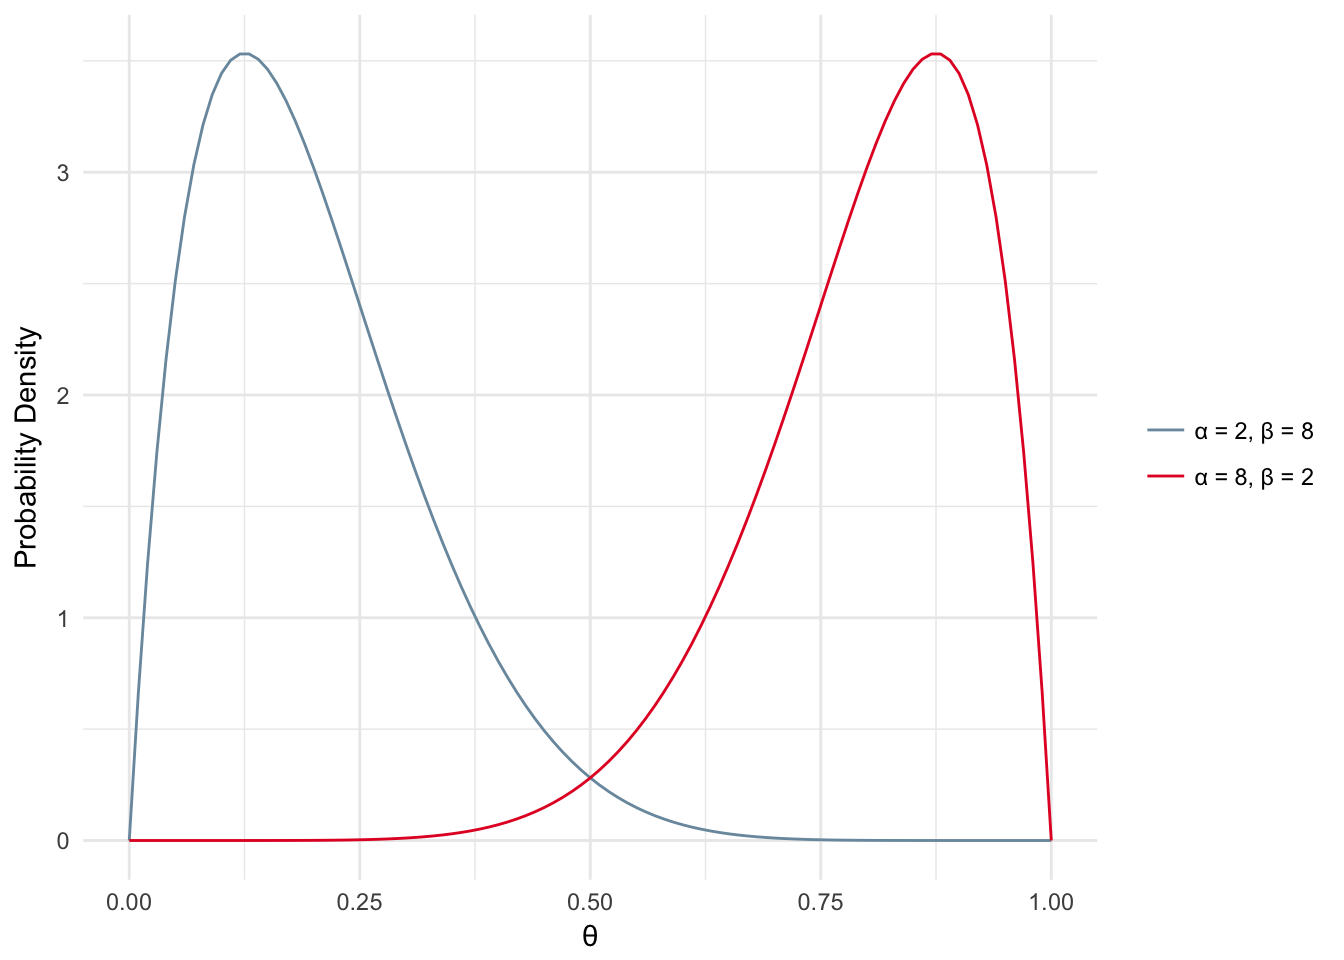
\includegraphics{_main_files/figure-latex/betaShapeSkewed-1.pdf}
\caption{\label{fig:betaShapeSkewed}Beta Distribution - Skewed}
\end{figure}

The probability distribution function for the beta distribution can be
found below.

\[
f(\theta;\alpha,\beta) ={{\theta^{(\alpha-1)}(1-\theta)^{(\beta-1)}}\over B(\alpha,\beta)}
\]

Quick Note:

\begin{itemize}
\tightlist
\item
  The \emph{Beta} function, \emph{B} is the ratio of the product of the
  \emph{Gamma} function, \(\Gamma\), of each parameter divided by the
  \emph{Gamma} function of the sum of the parameters. The \emph{Beta}
  function is \textbf{not} the same as the beta distribution. The
  \emph{Beta} function is shown below along with the \emph{Gamma}
  function, which is used in the \emph{Beta} function.
\end{itemize}

\[
\beta(a,b) = {\Gamma(a)\Gamma(b) \over{\Gamma(a+b)}}
\]

\begin{itemize}
\tightlist
\item
  The \emph{Gamma} function is the factorial of the parameter minus 1.
\end{itemize}

\[
\Gamma(a) = (a-1)!
\]

\section{Inference: The Building
Blocks}\label{inference-the-building-blocks}

The equation below is a fundamental to understanding parameter
estimation and inference.

\[
\underbrace{p(\theta|D)}_{posterior} = {\overbrace{p(D|\theta)}^{likelihood}
  \overbrace{p(\theta)}^{prior} \over \underbrace{p(D)}_{evidence}}
\tag{3}
\]

The 4 components are:

\begin{itemize}
\tightlist
\item
  \textbf{Prior}: The probability of the parameter(s). Defines our prior
  beliefs of the parameter. Do we \emph{believe} to a good degree of
  certainty that the coin is fair? Maybe take a step back and ask
  yourself `do I trust the manufacturer of this coin?'. If this
  manufacturer has always had great quality (i.e.~fair coins) then you
  would have some confidence that your case is no different.
\item
  \textbf{Posterior}: The probability of the parameter \textbf{given}
  the evidence. The only way to know this value is to already have the
  evidence. However we can estimate the posterior in various ways. Think
  of it this way, given 100 coin flips with 47 heads and 53 tails what
  is the probability that theta is 0.5 (coin is fair)?
\item
  \textbf{Likelihood}: The probability of the evidence \textbf{given}
  the parameter. Given that we know the coin is fair (theta = 0.5) what
  is the probability of having 47 heads out of 100 flips?
\item
  \textbf{Evidence}: The probability of all possible outcomes.
  Probability of 1/100 heads, 2/100 heads, \ldots{}, 100/100 heads.
\end{itemize}

\textbf{Conditioning your brain for LDA} : We are starting with a coin
flip, but the eventual goal is to link this back to words appearing in a
document. Try to keep in mind that we think of a word similar to the
outcome of a coin: a word exists in the document (heads!) or a word
doesn't exist in the document (tails!).

\section{Maximum Likelihood}\label{maximum-likelihood}

The simplest method of parameter estimation is the maximum likelihood
method. Effectively we calculate the parameter that maximizes the
likelihood.

\[ 
\underbrace{p(\theta|D)}_{posterior} = {\overbrace{\bf \Large p(D|\theta)}^{\bf \Large LIKELIHOOD}
  \overbrace{p(\theta)}^{prior} \over \underbrace{p(D)}_{evidence}}
\tag{4}
\]

Let's first discuss what the likelihood is. The likelihood can be
described as the probability of getting observed data given a specified
value of the parameter, \(\theta\). For example, let's say I've flipped
a coin 10 times and got 5 heads, 5 tails. Assuming the coin is fair,
\(\theta\) equals 0.5, what is the likelihood of observing 5 heads and 5
tails.

To calculate the likelihood of a parameter given a single outcome we
would use the probability mass function: \[
P(X=x)=\theta^{x}(1-\theta)^{1-x}, \hspace{1cm} x = \{0,1\} 
\tag{5}
\] Where an outcome of heads equal 1 and tails is 0. Now let's say we
have carried out the 10 flips as mentioned previously: \[
\begin{aligned}
P(X_{1}=x_{1},X_{2}=x_{2},...,X_{10}=x_{10}) &= \prod\limits_{n=1}^{10} \theta^{x}(1-\theta)^{1-x}\\
L(\theta) &= \prod\limits_{n=1}^{10} \theta^{x}(1-\theta)^{1-x}
\end{aligned}
\tag{6}
\] What is shown in the equations above is the joint probability mass
function. Each coin flip is independent so we calculate the product of
the PMF's for each trial. This is known as the likelihood function - the
likelihood of \(\theta\) given our observed data.

-------FIND A TEXT SOURCE-------
\url{https://onlinecourses.science.psu.edu/stat414/node/191}

Back to the maximum likelihood\ldots{}.

Our goal is to find the value of \(\theta\) which maximizes the
likelihood of the observed data. To derive the maximum likelihood we
start by taking the log of the likelihood, \(\mathcal{L}\).

\[
\begin{aligned}
\mathcal{L} &= log \prod\limits_{n=1}^N \theta^{x}(1-\theta)^{1-x} \\\\
 &= \sum\limits_{n=1}^N log(\theta^{x}(1-\theta)^{1-x}) \\\\
 &= n^{(1)}log(\theta) + n^{(0)}log(1-\theta)
\end{aligned}
\tag{7}
\] Differentiate with respect to \(\theta\):

\[
{d\mathcal{L} \over d\theta} =  {n^{(1)}\over \theta} - {n^{(0)}\over 1-\theta}
\tag{8}
\] Set it equal to zero and solve: \$\$

\begin{aligned}
{n^{(1)}\over \theta} - {n^{(0)}\over 1-\theta} &= 0  \\ \\
{n^{(1)}\over\theta} &= {n^{(0)}\over 1-\theta} \\ \\
{n^{1} - \theta n^{1}} &= {\theta n^{0}} \\ \\
n^{(1)} &= \theta(n^{(1)} + n^{0}) \\ \\
\theta &= {n^{(1)} \over N}
\end{aligned}

\tag{9}

\$\$

The value of \(\theta\) that maximizes the likelihood is the number of
heads over the number of flips.

\begin{Shaded}
\begin{Highlighting}[]
\NormalTok{heads =}\StringTok{ }\DecValTok{1}\OperatorTok{:}\DecValTok{10}
\NormalTok{flips =}\StringTok{ }\DecValTok{10}
\NormalTok{ds <-}\StringTok{ }\KeywordTok{data.frame}\NormalTok{(heads, }\DataTypeTok{flips =} \KeywordTok{rep}\NormalTok{(flips, }\KeywordTok{length}\NormalTok{(heads)))}
\NormalTok{ds}\OperatorTok{$}\NormalTok{theta <-}\StringTok{ }\NormalTok{ds}\OperatorTok{$}\NormalTok{heads}\OperatorTok{/}\NormalTok{ds}\OperatorTok{$}\NormalTok{flips}


\KeywordTok{ggplot}\NormalTok{(ds, }\KeywordTok{aes}\NormalTok{(}\DataTypeTok{x =}\NormalTok{ heads,}
               \DataTypeTok{y =}\NormalTok{ theta)) }\OperatorTok{+}\StringTok{ }
\StringTok{  }\KeywordTok{geom_point}\NormalTok{(}\DataTypeTok{color =}\StringTok{'#1520c1'}\NormalTok{, }\DataTypeTok{size =} \DecValTok{3}\NormalTok{) }\OperatorTok{+}\StringTok{ }
\StringTok{  }\KeywordTok{geom_linerange}\NormalTok{(}\KeywordTok{aes}\NormalTok{(}\DataTypeTok{x=}\NormalTok{heads,}
                     \DataTypeTok{y=}\OtherTok{NULL}\NormalTok{, }\DataTypeTok{ymax=}\NormalTok{theta,}
                     \DataTypeTok{ymin=}\DecValTok{0}\NormalTok{)) }\OperatorTok{+}
\StringTok{  }\KeywordTok{scale_x_continuous}\NormalTok{(}\DataTypeTok{breaks =} \KeywordTok{seq}\NormalTok{(}\DecValTok{0}\NormalTok{,}\DecValTok{10}\NormalTok{,}\DecValTok{2}\NormalTok{), }\DataTypeTok{labels =} \KeywordTok{seq}\NormalTok{(}\DecValTok{0}\NormalTok{,}\DecValTok{10}\NormalTok{,}\DecValTok{2}\NormalTok{)) }\OperatorTok{+}\StringTok{ }
\StringTok{  }\KeywordTok{labs}\NormalTok{(}\DataTypeTok{y=}\StringTok{'\textbackslash{}U03B8'}\NormalTok{, }\DataTypeTok{x=}\StringTok{"Number of Heads"}\NormalTok{, }\DataTypeTok{title =}\StringTok{"ML Parameter Estimation: 10 Bernoulli Trials"}\NormalTok{) }\OperatorTok{+}
\StringTok{  }\KeywordTok{theme}\NormalTok{(}\DataTypeTok{plot.title =} \KeywordTok{element_text}\NormalTok{(}\DataTypeTok{hjust =} \FloatTok{0.5}\NormalTok{)) }\OperatorTok{+}\StringTok{ }\KeywordTok{theme_minimal}\NormalTok{()}
\end{Highlighting}
\end{Shaded}

\begin{figure}
\centering
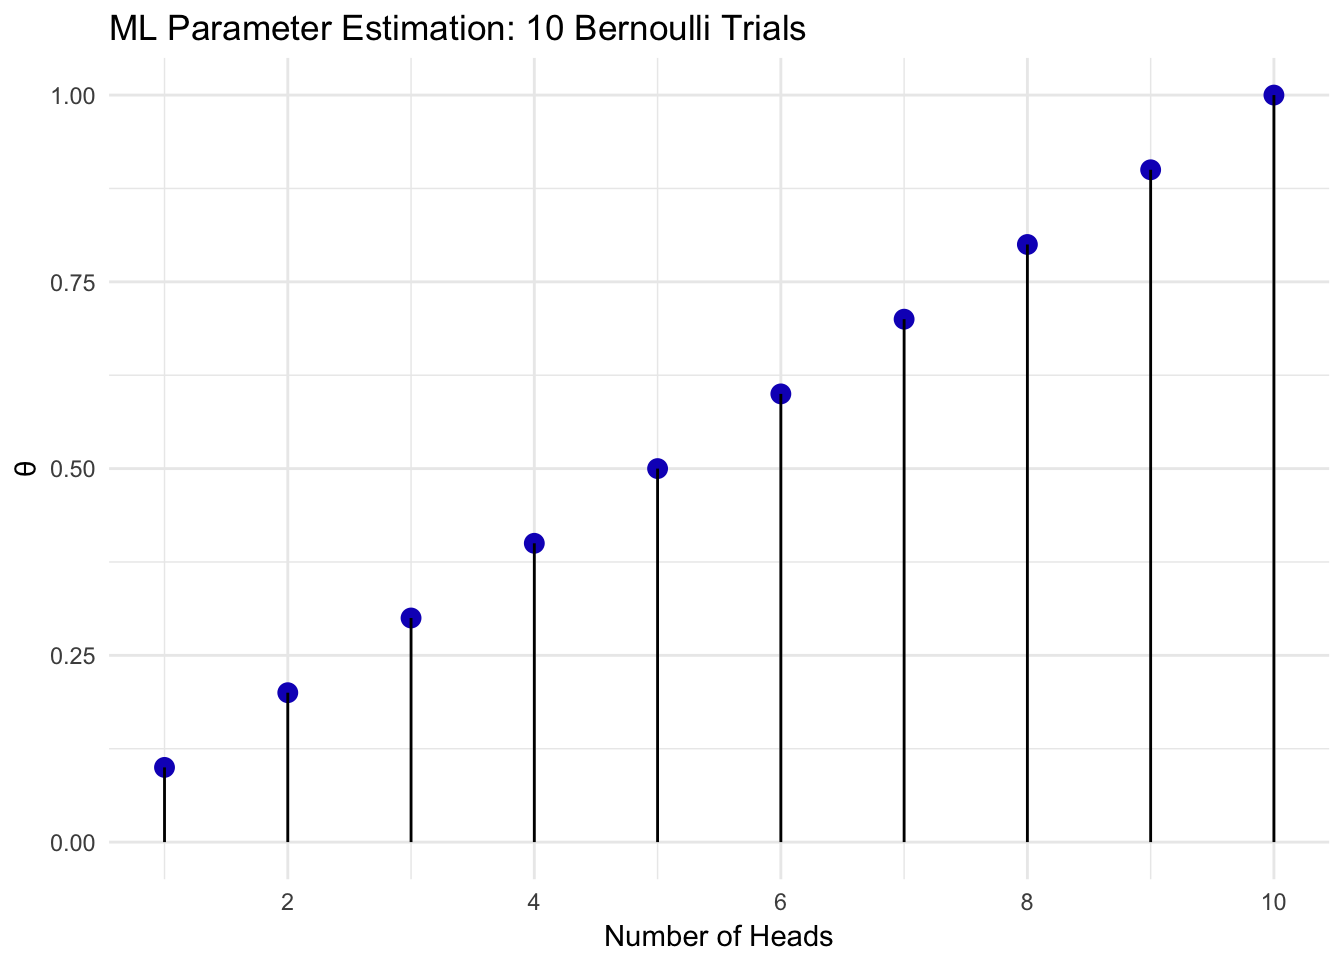
\includegraphics{_main_files/figure-latex/bernoulliml-1.pdf}
\caption{\label{fig:bernoulliml}Bernoulli Maximum Likelihood}
\end{figure}

\section{Maximum a Posteriori (MAP)}\label{maximum-a-posteriori-map}

MAP is similar to the method of maximum likelihood estimation, but it
also let's us include information about our prior beliefs. Unlike ML
estimation, MAP estimates parameters by trying to maximize the
posterior.

\[
\theta_{MAP}=\underset{\theta}{\operatorname{argmax}} P(\theta|X)
\tag{10}
\]

\[
\require{enclose}
\theta_{MAP}=\underset{\theta}{\operatorname{argmax}}{\overbrace{p(D|\theta)}^{likelihood}
  \overbrace{p(\theta)}^{prior} \over \underbrace{\enclose{horizontalstrike}{p(D)}}_{evidence}}
\tag{11}
\]

The evidence term is dropped during the calculation of \(\theta_{MAP}\)
since it is not a function of \(\theta\) and our only concern is
maximizing the posterior based on \(\theta\). Similar to calculating the
Likelhood, the first step is to apply the log function to the remaining
terms.

\[
\begin{aligned}
\theta_{MAP} &=\underset{\theta}{\operatorname{argmax}}p(D|\theta)p(\theta) \\\\
&= \mathcal{L}(\theta|D) + log(p(\theta))
\end{aligned}
\tag{12}
\]

We have already derived the log likelihood during our derivation of the
maximum likelihood, so let's now focus on the prior. The prior for the
Bernoulli distribution is the Beta distribution and can be used to
describe \(p(\theta)\). The probability distribution function, PDF, for
the Beta distribution is shown below.

\[
p(\theta|\alpha,\beta) = {\theta^{\alpha-1}(1-\theta)^{\beta-1}\over{B(\alpha, \beta)}}
\tag{13}
\] Plugging in the PDF of the beta distribution for the prior:

\$\$

\begin{aligned}
\theta_{MAP}&= \mathcal{L}(\theta|D) + log(p(\theta)) \\\\
\theta_{MAP}&= n^{(1)}log(\theta) + n^{(0)}log(1-\theta) + log({\theta^{\alpha-1}(1-\theta)^{\beta-1}\over{B(\alpha, \beta)}}) \\\\
\theta_{MAP}&= n^{(1)}log(\theta) + n^{(0)}log(1-\theta) + log({\theta^{\alpha-1}) + log((1-\theta)^{\beta-1})-log({B(\alpha, \beta)}}) \\\\


{d \over d\theta} \mathcal{L}(\theta|D) + log(p(\theta)) &= {n^{(1)}\over \theta} - {n^{(0)}\over 1-\theta} + {\alpha - 1\over\theta} - {\beta - 1 \over 1-\theta}
\\\\
0 &= {n^{(1)}\over \theta} - {n^{(0)}\over 1-\theta} + {\alpha - 1\over\theta} - {\beta - 1 \over 1-\theta}
\\\\
\theta_{MAP}&= {{n^{(1)} + \alpha -1} \over {n^{(1)} + n^{0} + \alpha + \beta - 2}}
\end{aligned}

\tag{14} \$\$

Now that we know how to calculate the parameter \(\theta\) that
maximizes the posterior, lets take a look at how choices of different
priors effects our outcome.

\begin{Shaded}
\begin{Highlighting}[]
\CommentTok{# description:}
\CommentTok{# ml will yeild the expected average and is not effected by the prior}
\CommentTok{# map uses a weak assumption - uniform density for all values of theta}
\CommentTok{# this results in a theta_map value very similar to the ml value}
\NormalTok{n <-}\StringTok{ }\DecValTok{20}
\NormalTok{heads <-}\StringTok{ }\DecValTok{12}
\NormalTok{tails <-}\StringTok{ }\DecValTok{8}


\CommentTok{# ml}
\NormalTok{ml_theta <-}\StringTok{ }\NormalTok{heads}\OperatorTok{/}\NormalTok{n}
\CommentTok{# map}
\NormalTok{B <-}\StringTok{ }\DecValTok{2}
\NormalTok{alpha <-}\StringTok{ }\DecValTok{2}

\NormalTok{map_theta <-}\StringTok{ }\NormalTok{(heads }\OperatorTok{+}\StringTok{ }\NormalTok{alpha }\OperatorTok{-}\StringTok{ }\DecValTok{1}\NormalTok{)}\OperatorTok{/}\NormalTok{(heads }\OperatorTok{+}\StringTok{ }\NormalTok{tails }\OperatorTok{+}\StringTok{ }\NormalTok{alpha }\OperatorTok{+}\StringTok{ }\NormalTok{B }\OperatorTok{-}\DecValTok{2}\NormalTok{)}
\NormalTok{possible_theta <-}\StringTok{ }\KeywordTok{seq}\NormalTok{(}\DecValTok{0}\NormalTok{,}\DecValTok{1}\NormalTok{,}\FloatTok{0.01}\NormalTok{)}
\NormalTok{beta_ds <-}\StringTok{ }\KeywordTok{data.frame}\NormalTok{(}\DataTypeTok{theta =}\NormalTok{ possible_theta, }\DataTypeTok{density =} \KeywordTok{dbeta}\NormalTok{(possible_theta, alpha,B))}
\KeywordTok{ggplot}\NormalTok{(beta_ds, }\KeywordTok{aes}\NormalTok{(}\DataTypeTok{x =}\NormalTok{ theta, }\DataTypeTok{y =}\NormalTok{ density)) }\OperatorTok{+}\StringTok{ }\KeywordTok{geom_point}\NormalTok{(}\DataTypeTok{color=}\StringTok{'#7A99AC'}\NormalTok{) }\OperatorTok{+}\StringTok{ }
\StringTok{  }\KeywordTok{geom_vline}\NormalTok{(}\DataTypeTok{xintercept=}\NormalTok{map_theta, }\DataTypeTok{color =} \StringTok{'#ba0223'}\NormalTok{) }\OperatorTok{+}\StringTok{ }
\StringTok{  }\KeywordTok{annotate}\NormalTok{(}\StringTok{"text"}\NormalTok{, }\DataTypeTok{x =}\NormalTok{ map_theta }\OperatorTok{+}\StringTok{ }\FloatTok{0.1}\NormalTok{, }\DataTypeTok{y=}\FloatTok{0.5}\NormalTok{, }\DataTypeTok{label=} \KeywordTok{paste}\NormalTok{(}\StringTok{"\textbackslash{}U03B8[MAP]=="}\NormalTok{, }\KeywordTok{round}\NormalTok{(map_theta,}\DecValTok{2}\NormalTok{)), }\DataTypeTok{parse=}\NormalTok{T)}\OperatorTok{+}
\StringTok{  }\KeywordTok{labs}\NormalTok{(}\DataTypeTok{x=}\StringTok{'\textbackslash{}U03B8'}\NormalTok{) }\OperatorTok{+}\StringTok{ }\KeywordTok{theme_minimal}\NormalTok{()}
\end{Highlighting}
\end{Shaded}

\begin{verbatim}
## Warning in grid.Call(C_stringMetric, as.graphicsAnnot(x$label)): font
## metrics unknown for Unicode character U+03b8

## Warning in grid.Call(C_stringMetric, as.graphicsAnnot(x$label)): font
## metrics unknown for Unicode character U+03b8
\end{verbatim}

\begin{verbatim}
## Warning in grid.Call(C_stringMetric, as.graphicsAnnot(x$label)): conversion
## failure on 'θ' in 'mbcsToSbcs': dot substituted for <ce>
\end{verbatim}

\begin{verbatim}
## Warning in grid.Call(C_stringMetric, as.graphicsAnnot(x$label)): conversion
## failure on 'θ' in 'mbcsToSbcs': dot substituted for <b8>
\end{verbatim}

\begin{verbatim}
## Warning in grid.Call(C_textBounds, as.graphicsAnnot(x$label), x$x, x$y, :
## conversion failure on 'θ' in 'mbcsToSbcs': dot substituted for <ce>
\end{verbatim}

\begin{verbatim}
## Warning in grid.Call(C_textBounds, as.graphicsAnnot(x$label), x$x, x$y, :
## conversion failure on 'θ' in 'mbcsToSbcs': dot substituted for <b8>
\end{verbatim}

\begin{verbatim}
## Warning in grid.Call(C_textBounds, as.graphicsAnnot(x$label), x$x, x$y, :
## conversion failure on 'θ' in 'mbcsToSbcs': dot substituted for <ce>
\end{verbatim}

\begin{verbatim}
## Warning in grid.Call(C_textBounds, as.graphicsAnnot(x$label), x$x, x$y, :
## conversion failure on 'θ' in 'mbcsToSbcs': dot substituted for <b8>
\end{verbatim}

\begin{verbatim}
## Warning in grid.Call(C_textBounds, as.graphicsAnnot(x$label), x$x, x$y, :
## conversion failure on 'θ' in 'mbcsToSbcs': dot substituted for <ce>
\end{verbatim}

\begin{verbatim}
## Warning in grid.Call(C_textBounds, as.graphicsAnnot(x$label), x$x, x$y, :
## conversion failure on 'θ' in 'mbcsToSbcs': dot substituted for <b8>
\end{verbatim}

\begin{verbatim}
## Warning in grid.Call(C_textBounds, as.graphicsAnnot(x$label), x$x, x$y, :
## conversion failure on 'θ' in 'mbcsToSbcs': dot substituted for <ce>
\end{verbatim}

\begin{verbatim}
## Warning in grid.Call(C_textBounds, as.graphicsAnnot(x$label), x$x, x$y, :
## conversion failure on 'θ' in 'mbcsToSbcs': dot substituted for <b8>
\end{verbatim}

\begin{verbatim}
## Warning in grid.Call(C_textBounds, as.graphicsAnnot(x$label), x$x, x$y, :
## conversion failure on 'θ' in 'mbcsToSbcs': dot substituted for <ce>
\end{verbatim}

\begin{verbatim}
## Warning in grid.Call(C_textBounds, as.graphicsAnnot(x$label), x$x, x$y, :
## conversion failure on 'θ' in 'mbcsToSbcs': dot substituted for <b8>
\end{verbatim}

\begin{verbatim}
## Warning in grid.Call.graphics(C_text, as.graphicsAnnot(x$label), x$x, x
## $y, : font metrics unknown for Unicode character U+03b8

## Warning in grid.Call.graphics(C_text, as.graphicsAnnot(x$label), x$x, x
## $y, : font metrics unknown for Unicode character U+03b8
\end{verbatim}

\begin{verbatim}
## Warning in grid.Call.graphics(C_text, as.graphicsAnnot(x$label), x$x, x
## $y, : conversion failure on 'θ' in 'mbcsToSbcs': dot substituted for <ce>
\end{verbatim}

\begin{verbatim}
## Warning in grid.Call.graphics(C_text, as.graphicsAnnot(x$label), x$x, x
## $y, : conversion failure on 'θ' in 'mbcsToSbcs': dot substituted for <b8>
\end{verbatim}

\begin{verbatim}
## Warning in grid.Call(C_textBounds, as.graphicsAnnot(x$label), x$x, x$y, :
## conversion failure on 'θ' in 'mbcsToSbcs': dot substituted for <ce>
\end{verbatim}

\begin{verbatim}
## Warning in grid.Call(C_textBounds, as.graphicsAnnot(x$label), x$x, x$y, :
## conversion failure on 'θ' in 'mbcsToSbcs': dot substituted for <b8>
\end{verbatim}

\begin{verbatim}
## Warning in grid.Call(C_textBounds, as.graphicsAnnot(x$label), x$x, x$y, :
## conversion failure on 'θ' in 'mbcsToSbcs': dot substituted for <ce>
\end{verbatim}

\begin{verbatim}
## Warning in grid.Call(C_textBounds, as.graphicsAnnot(x$label), x$x, x$y, :
## conversion failure on 'θ' in 'mbcsToSbcs': dot substituted for <b8>
\end{verbatim}

\begin{verbatim}
## Warning in grid.Call.graphics(C_text, as.graphicsAnnot(x$label), x$x, x
## $y, : conversion failure on 'θ' in 'mbcsToSbcs': dot substituted for <ce>
\end{verbatim}

\begin{verbatim}
## Warning in grid.Call.graphics(C_text, as.graphicsAnnot(x$label), x$x, x
## $y, : conversion failure on 'θ' in 'mbcsToSbcs': dot substituted for <b8>
\end{verbatim}

\begin{figure}
\centering
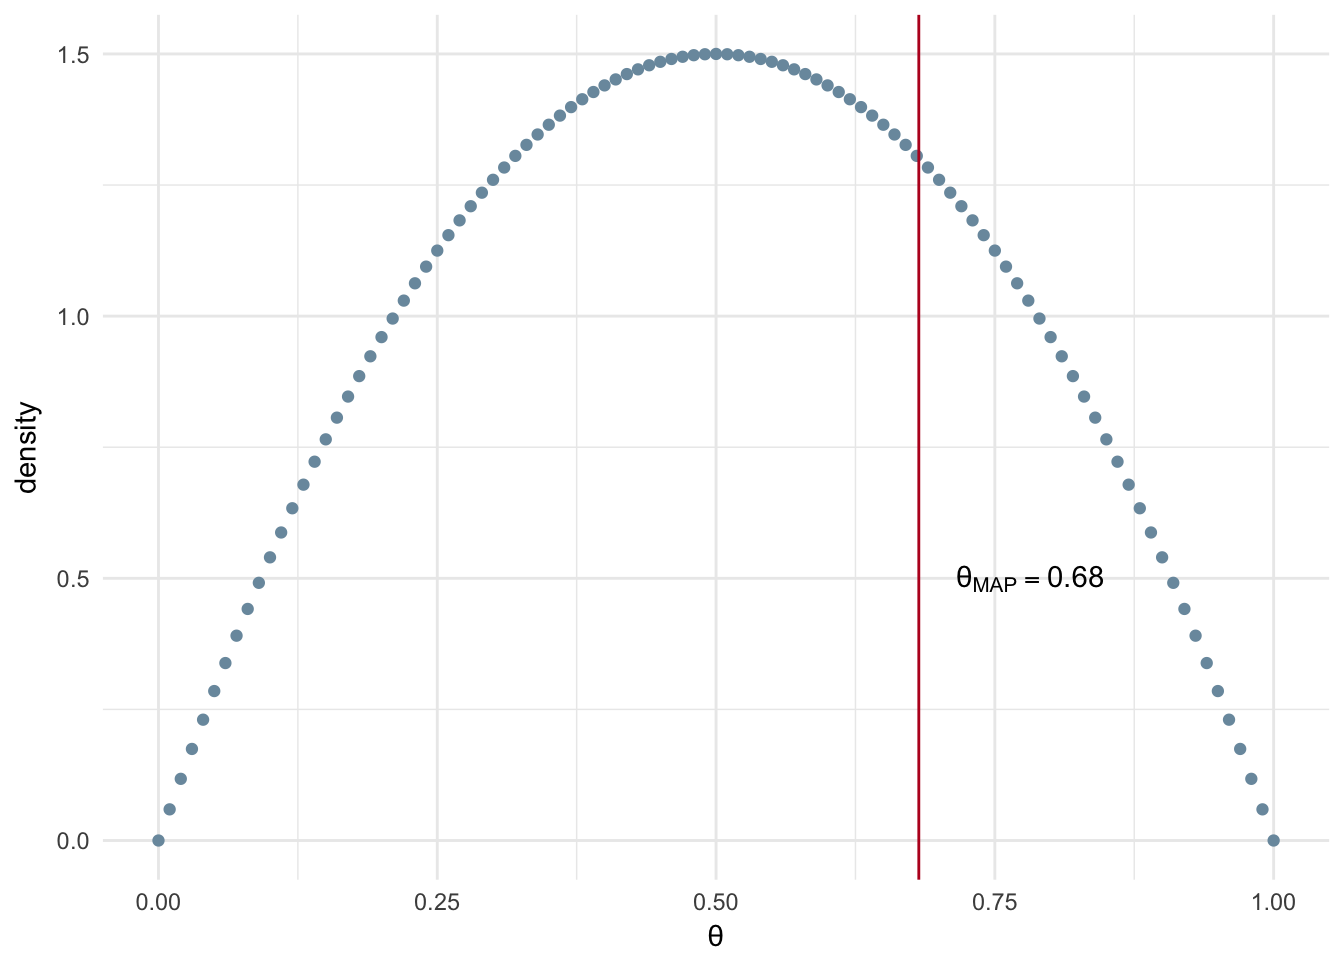
\includegraphics{_main_files/figure-latex/mapSmallnUninformedPrior-1.pdf}
\caption{\label{fig:mapSmallnUninformedPrior}MAP: Small number of
experiments and uninformed prior}
\end{figure}

\begin{Shaded}
\begin{Highlighting}[]
\CommentTok{# description:}
\CommentTok{# the strong assumption of a 'fair' coin prior reduces the width of the }
\CommentTok{# distribution, i.e. much higher probability density near theta (p) of 0.5}
\CommentTok{# This forces the MAP theta value to stay much closer to the prior due to the }
\CommentTok{# small amount of observed evidence}

\NormalTok{n <-}\StringTok{ }\DecValTok{20}
\NormalTok{heads <-}\StringTok{ }\DecValTok{12}
\NormalTok{tails <-}\StringTok{ }\DecValTok{8}


\CommentTok{# ml}
\NormalTok{ml_theta <-}\StringTok{ }\NormalTok{heads}\OperatorTok{/}\NormalTok{n}
\CommentTok{# map}
\NormalTok{B <-}\StringTok{ }\DecValTok{100}
\NormalTok{alpha <-}\StringTok{ }\DecValTok{100}

\NormalTok{map_theta <-}\StringTok{ }\NormalTok{(heads }\OperatorTok{+}\StringTok{ }\NormalTok{alpha }\OperatorTok{-}\StringTok{ }\DecValTok{1}\NormalTok{)}\OperatorTok{/}\NormalTok{(heads }\OperatorTok{+}\StringTok{ }\NormalTok{tails }\OperatorTok{+}\StringTok{ }\NormalTok{alpha }\OperatorTok{+}\StringTok{ }\NormalTok{B }\OperatorTok{-}\DecValTok{2}\NormalTok{)}
\NormalTok{possible_theta <-}\StringTok{ }\KeywordTok{seq}\NormalTok{(}\DecValTok{0}\NormalTok{,}\DecValTok{1}\NormalTok{,}\FloatTok{0.001}\NormalTok{)}
\NormalTok{beta_ds <-}\StringTok{ }\KeywordTok{data.frame}\NormalTok{(}\DataTypeTok{theta =}\NormalTok{ possible_theta, }\DataTypeTok{density =} \KeywordTok{dbeta}\NormalTok{(possible_theta, alpha,B))}
\KeywordTok{ggplot}\NormalTok{(beta_ds, }\KeywordTok{aes}\NormalTok{(}\DataTypeTok{x =}\NormalTok{ theta, }\DataTypeTok{y =}\NormalTok{ density)) }\OperatorTok{+}\StringTok{ }\KeywordTok{geom_line}\NormalTok{(}\DataTypeTok{color=}\StringTok{'#7A99AC'}\NormalTok{) }\OperatorTok{+}\StringTok{ }
\StringTok{  }\KeywordTok{geom_vline}\NormalTok{(}\DataTypeTok{xintercept=}\NormalTok{map_theta, }\DataTypeTok{color =} \StringTok{'#ba0223'}\NormalTok{) }\OperatorTok{+}\StringTok{ }
\StringTok{  }\KeywordTok{annotate}\NormalTok{(}\StringTok{"text"}\NormalTok{, }\DataTypeTok{x =}\NormalTok{ map_theta }\OperatorTok{+}\StringTok{ }\FloatTok{0.1}\NormalTok{, }\DataTypeTok{y=}\DecValTok{11}\NormalTok{, }\DataTypeTok{label=} \KeywordTok{paste}\NormalTok{(}\StringTok{"\textbackslash{}U03B8[MAP]=="}\NormalTok{, }\KeywordTok{round}\NormalTok{(map_theta,}\DecValTok{2}\NormalTok{)), }\DataTypeTok{parse=}\NormalTok{T)}\OperatorTok{+}
\StringTok{  }\KeywordTok{labs}\NormalTok{(}\DataTypeTok{x=}\StringTok{'\textbackslash{}U03B8'}\NormalTok{, }\DataTypeTok{y =} \StringTok{'Density'}\NormalTok{) }\OperatorTok{+}\StringTok{ }\KeywordTok{theme_minimal}\NormalTok{()}
\end{Highlighting}
\end{Shaded}

\begin{verbatim}
## Warning in grid.Call(C_stringMetric, as.graphicsAnnot(x$label)): font
## metrics unknown for Unicode character U+03b8

## Warning in grid.Call(C_stringMetric, as.graphicsAnnot(x$label)): font
## metrics unknown for Unicode character U+03b8
\end{verbatim}

\begin{verbatim}
## Warning in grid.Call(C_stringMetric, as.graphicsAnnot(x$label)): conversion
## failure on 'θ' in 'mbcsToSbcs': dot substituted for <ce>
\end{verbatim}

\begin{verbatim}
## Warning in grid.Call(C_stringMetric, as.graphicsAnnot(x$label)): conversion
## failure on 'θ' in 'mbcsToSbcs': dot substituted for <b8>
\end{verbatim}

\begin{verbatim}
## Warning in grid.Call(C_textBounds, as.graphicsAnnot(x$label), x$x, x$y, :
## conversion failure on 'θ' in 'mbcsToSbcs': dot substituted for <ce>
\end{verbatim}

\begin{verbatim}
## Warning in grid.Call(C_textBounds, as.graphicsAnnot(x$label), x$x, x$y, :
## conversion failure on 'θ' in 'mbcsToSbcs': dot substituted for <b8>
\end{verbatim}

\begin{verbatim}
## Warning in grid.Call(C_textBounds, as.graphicsAnnot(x$label), x$x, x$y, :
## conversion failure on 'θ' in 'mbcsToSbcs': dot substituted for <ce>
\end{verbatim}

\begin{verbatim}
## Warning in grid.Call(C_textBounds, as.graphicsAnnot(x$label), x$x, x$y, :
## conversion failure on 'θ' in 'mbcsToSbcs': dot substituted for <b8>
\end{verbatim}

\begin{verbatim}
## Warning in grid.Call(C_textBounds, as.graphicsAnnot(x$label), x$x, x$y, :
## conversion failure on 'θ' in 'mbcsToSbcs': dot substituted for <ce>
\end{verbatim}

\begin{verbatim}
## Warning in grid.Call(C_textBounds, as.graphicsAnnot(x$label), x$x, x$y, :
## conversion failure on 'θ' in 'mbcsToSbcs': dot substituted for <b8>
\end{verbatim}

\begin{verbatim}
## Warning in grid.Call(C_textBounds, as.graphicsAnnot(x$label), x$x, x$y, :
## conversion failure on 'θ' in 'mbcsToSbcs': dot substituted for <ce>
\end{verbatim}

\begin{verbatim}
## Warning in grid.Call(C_textBounds, as.graphicsAnnot(x$label), x$x, x$y, :
## conversion failure on 'θ' in 'mbcsToSbcs': dot substituted for <b8>
\end{verbatim}

\begin{verbatim}
## Warning in grid.Call(C_textBounds, as.graphicsAnnot(x$label), x$x, x$y, :
## conversion failure on 'θ' in 'mbcsToSbcs': dot substituted for <ce>
\end{verbatim}

\begin{verbatim}
## Warning in grid.Call(C_textBounds, as.graphicsAnnot(x$label), x$x, x$y, :
## conversion failure on 'θ' in 'mbcsToSbcs': dot substituted for <b8>
\end{verbatim}

\begin{verbatim}
## Warning in grid.Call.graphics(C_text, as.graphicsAnnot(x$label), x$x, x
## $y, : font metrics unknown for Unicode character U+03b8

## Warning in grid.Call.graphics(C_text, as.graphicsAnnot(x$label), x$x, x
## $y, : font metrics unknown for Unicode character U+03b8
\end{verbatim}

\begin{verbatim}
## Warning in grid.Call.graphics(C_text, as.graphicsAnnot(x$label), x$x, x
## $y, : conversion failure on 'θ' in 'mbcsToSbcs': dot substituted for <ce>
\end{verbatim}

\begin{verbatim}
## Warning in grid.Call.graphics(C_text, as.graphicsAnnot(x$label), x$x, x
## $y, : conversion failure on 'θ' in 'mbcsToSbcs': dot substituted for <b8>
\end{verbatim}

\begin{verbatim}
## Warning in grid.Call(C_textBounds, as.graphicsAnnot(x$label), x$x, x$y, :
## conversion failure on 'θ' in 'mbcsToSbcs': dot substituted for <ce>
\end{verbatim}

\begin{verbatim}
## Warning in grid.Call(C_textBounds, as.graphicsAnnot(x$label), x$x, x$y, :
## conversion failure on 'θ' in 'mbcsToSbcs': dot substituted for <b8>
\end{verbatim}

\begin{verbatim}
## Warning in grid.Call(C_textBounds, as.graphicsAnnot(x$label), x$x, x$y, :
## conversion failure on 'θ' in 'mbcsToSbcs': dot substituted for <ce>
\end{verbatim}

\begin{verbatim}
## Warning in grid.Call(C_textBounds, as.graphicsAnnot(x$label), x$x, x$y, :
## conversion failure on 'θ' in 'mbcsToSbcs': dot substituted for <b8>
\end{verbatim}

\begin{verbatim}
## Warning in grid.Call.graphics(C_text, as.graphicsAnnot(x$label), x$x, x
## $y, : conversion failure on 'θ' in 'mbcsToSbcs': dot substituted for <ce>
\end{verbatim}

\begin{verbatim}
## Warning in grid.Call.graphics(C_text, as.graphicsAnnot(x$label), x$x, x
## $y, : conversion failure on 'θ' in 'mbcsToSbcs': dot substituted for <b8>
\end{verbatim}

\begin{figure}
\centering
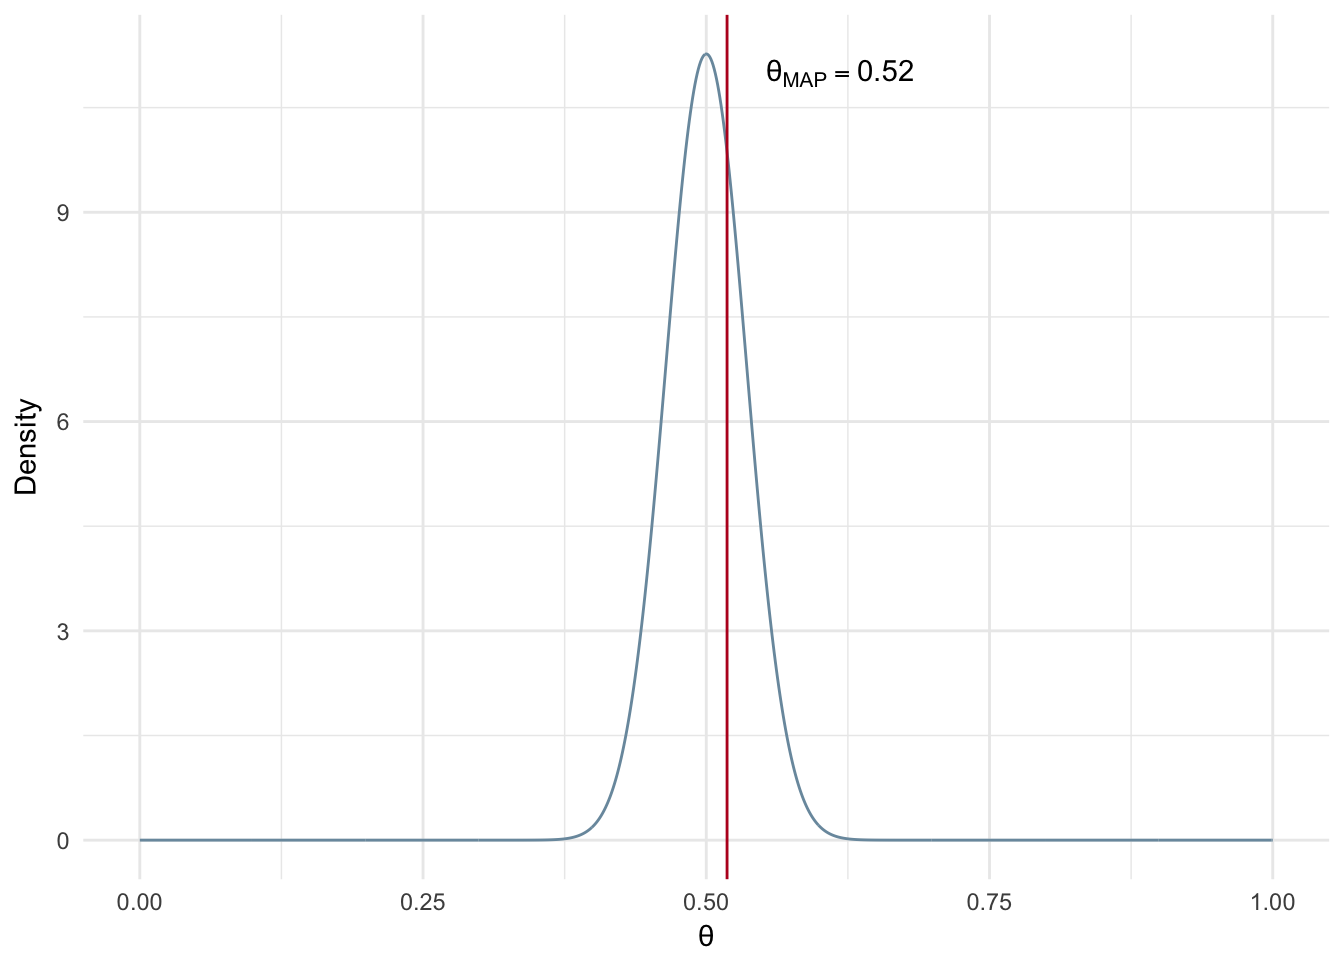
\includegraphics{_main_files/figure-latex/mapSmallnInformedPrior-1.pdf}
\caption{\label{fig:mapSmallnInformedPrior}MAP: Small number of experiments
and informed prior}
\end{figure}

\begin{Shaded}
\begin{Highlighting}[]
\CommentTok{# description}
\CommentTok{# high number of observed samples (evidence)}
\CommentTok{# weak prior - uniform }
\CommentTok{# ml and map are close to one another - close... as expected}
\NormalTok{n <-}\StringTok{ }\DecValTok{1000}
\NormalTok{heads <-}\StringTok{ }\DecValTok{723}
\NormalTok{tails <-}\StringTok{ }\NormalTok{n}\OperatorTok{-}\NormalTok{heads}


\CommentTok{# ml}
\NormalTok{ml_theta <-}\StringTok{ }\NormalTok{heads}\OperatorTok{/}\NormalTok{n}
\CommentTok{# map}
\NormalTok{B <-}\StringTok{ }\DecValTok{2}
\NormalTok{alpha <-}\StringTok{ }\DecValTok{2}
\NormalTok{map_theta <-}\StringTok{ }\NormalTok{(heads }\OperatorTok{+}\StringTok{ }\NormalTok{alpha }\OperatorTok{-}\StringTok{ }\DecValTok{1}\NormalTok{)}\OperatorTok{/}\NormalTok{(heads }\OperatorTok{+}\StringTok{ }\NormalTok{tails }\OperatorTok{+}\StringTok{ }\NormalTok{alpha }\OperatorTok{+}\StringTok{ }\NormalTok{B }\OperatorTok{-}\DecValTok{2}\NormalTok{)}
\NormalTok{possible_theta <-}\StringTok{ }\KeywordTok{seq}\NormalTok{(}\DecValTok{0}\NormalTok{,}\DecValTok{1}\NormalTok{,}\FloatTok{0.001}\NormalTok{)}
\NormalTok{beta_ds <-}\StringTok{ }\KeywordTok{data.frame}\NormalTok{(}\DataTypeTok{theta =}\NormalTok{ possible_theta, }\DataTypeTok{density =} \KeywordTok{dbeta}\NormalTok{(possible_theta, alpha,B))}
\KeywordTok{ggplot}\NormalTok{(beta_ds, }\KeywordTok{aes}\NormalTok{(}\DataTypeTok{x =}\NormalTok{ theta, }\DataTypeTok{y =}\NormalTok{ density)) }\OperatorTok{+}\StringTok{ }\KeywordTok{geom_line}\NormalTok{(}\DataTypeTok{color=}\StringTok{'#7A99AC'}\NormalTok{) }\OperatorTok{+}\StringTok{ }
\StringTok{  }\KeywordTok{geom_vline}\NormalTok{(}\DataTypeTok{xintercept=}\NormalTok{map_theta, }\DataTypeTok{color =} \StringTok{'#ba0223'}\NormalTok{) }\OperatorTok{+}\StringTok{ }
\StringTok{  }\KeywordTok{annotate}\NormalTok{(}\StringTok{"text"}\NormalTok{, }\DataTypeTok{x =}\NormalTok{ map_theta }\OperatorTok{+}\StringTok{ }\FloatTok{0.2}\NormalTok{, }\DataTypeTok{y=}\FloatTok{1.2}\NormalTok{, }\DataTypeTok{label=} \KeywordTok{paste}\NormalTok{(}\StringTok{"\textbackslash{}U03B8[MAP]=="}\NormalTok{, }\KeywordTok{round}\NormalTok{(map_theta,}\DecValTok{2}\NormalTok{)), }\DataTypeTok{parse=}\NormalTok{T)}\OperatorTok{+}
\StringTok{  }\KeywordTok{labs}\NormalTok{(}\DataTypeTok{x=}\StringTok{'\textbackslash{}U03B8'}\NormalTok{, }\DataTypeTok{y =} \StringTok{'Density'}\NormalTok{) }\OperatorTok{+}\StringTok{ }\KeywordTok{theme_minimal}\NormalTok{()}
\end{Highlighting}
\end{Shaded}

\begin{verbatim}
## Warning in grid.Call(C_stringMetric, as.graphicsAnnot(x$label)): font
## metrics unknown for Unicode character U+03b8

## Warning in grid.Call(C_stringMetric, as.graphicsAnnot(x$label)): font
## metrics unknown for Unicode character U+03b8
\end{verbatim}

\begin{verbatim}
## Warning in grid.Call(C_stringMetric, as.graphicsAnnot(x$label)): conversion
## failure on 'θ' in 'mbcsToSbcs': dot substituted for <ce>
\end{verbatim}

\begin{verbatim}
## Warning in grid.Call(C_stringMetric, as.graphicsAnnot(x$label)): conversion
## failure on 'θ' in 'mbcsToSbcs': dot substituted for <b8>
\end{verbatim}

\begin{verbatim}
## Warning in grid.Call(C_textBounds, as.graphicsAnnot(x$label), x$x, x$y, :
## conversion failure on 'θ' in 'mbcsToSbcs': dot substituted for <ce>
\end{verbatim}

\begin{verbatim}
## Warning in grid.Call(C_textBounds, as.graphicsAnnot(x$label), x$x, x$y, :
## conversion failure on 'θ' in 'mbcsToSbcs': dot substituted for <b8>
\end{verbatim}

\begin{verbatim}
## Warning in grid.Call(C_textBounds, as.graphicsAnnot(x$label), x$x, x$y, :
## conversion failure on 'θ' in 'mbcsToSbcs': dot substituted for <ce>
\end{verbatim}

\begin{verbatim}
## Warning in grid.Call(C_textBounds, as.graphicsAnnot(x$label), x$x, x$y, :
## conversion failure on 'θ' in 'mbcsToSbcs': dot substituted for <b8>
\end{verbatim}

\begin{verbatim}
## Warning in grid.Call(C_textBounds, as.graphicsAnnot(x$label), x$x, x$y, :
## conversion failure on 'θ' in 'mbcsToSbcs': dot substituted for <ce>
\end{verbatim}

\begin{verbatim}
## Warning in grid.Call(C_textBounds, as.graphicsAnnot(x$label), x$x, x$y, :
## conversion failure on 'θ' in 'mbcsToSbcs': dot substituted for <b8>
\end{verbatim}

\begin{verbatim}
## Warning in grid.Call(C_textBounds, as.graphicsAnnot(x$label), x$x, x$y, :
## conversion failure on 'θ' in 'mbcsToSbcs': dot substituted for <ce>
\end{verbatim}

\begin{verbatim}
## Warning in grid.Call(C_textBounds, as.graphicsAnnot(x$label), x$x, x$y, :
## conversion failure on 'θ' in 'mbcsToSbcs': dot substituted for <b8>
\end{verbatim}

\begin{verbatim}
## Warning in grid.Call(C_textBounds, as.graphicsAnnot(x$label), x$x, x$y, :
## conversion failure on 'θ' in 'mbcsToSbcs': dot substituted for <ce>
\end{verbatim}

\begin{verbatim}
## Warning in grid.Call(C_textBounds, as.graphicsAnnot(x$label), x$x, x$y, :
## conversion failure on 'θ' in 'mbcsToSbcs': dot substituted for <b8>
\end{verbatim}

\begin{verbatim}
## Warning in grid.Call.graphics(C_text, as.graphicsAnnot(x$label), x$x, x
## $y, : font metrics unknown for Unicode character U+03b8

## Warning in grid.Call.graphics(C_text, as.graphicsAnnot(x$label), x$x, x
## $y, : font metrics unknown for Unicode character U+03b8
\end{verbatim}

\begin{verbatim}
## Warning in grid.Call.graphics(C_text, as.graphicsAnnot(x$label), x$x, x
## $y, : conversion failure on 'θ' in 'mbcsToSbcs': dot substituted for <ce>
\end{verbatim}

\begin{verbatim}
## Warning in grid.Call.graphics(C_text, as.graphicsAnnot(x$label), x$x, x
## $y, : conversion failure on 'θ' in 'mbcsToSbcs': dot substituted for <b8>
\end{verbatim}

\begin{verbatim}
## Warning in grid.Call(C_textBounds, as.graphicsAnnot(x$label), x$x, x$y, :
## conversion failure on 'θ' in 'mbcsToSbcs': dot substituted for <ce>
\end{verbatim}

\begin{verbatim}
## Warning in grid.Call(C_textBounds, as.graphicsAnnot(x$label), x$x, x$y, :
## conversion failure on 'θ' in 'mbcsToSbcs': dot substituted for <b8>
\end{verbatim}

\begin{verbatim}
## Warning in grid.Call(C_textBounds, as.graphicsAnnot(x$label), x$x, x$y, :
## conversion failure on 'θ' in 'mbcsToSbcs': dot substituted for <ce>
\end{verbatim}

\begin{verbatim}
## Warning in grid.Call(C_textBounds, as.graphicsAnnot(x$label), x$x, x$y, :
## conversion failure on 'θ' in 'mbcsToSbcs': dot substituted for <b8>
\end{verbatim}

\begin{verbatim}
## Warning in grid.Call.graphics(C_text, as.graphicsAnnot(x$label), x$x, x
## $y, : conversion failure on 'θ' in 'mbcsToSbcs': dot substituted for <ce>
\end{verbatim}

\begin{verbatim}
## Warning in grid.Call.graphics(C_text, as.graphicsAnnot(x$label), x$x, x
## $y, : conversion failure on 'θ' in 'mbcsToSbcs': dot substituted for <b8>
\end{verbatim}

\begin{figure}
\centering
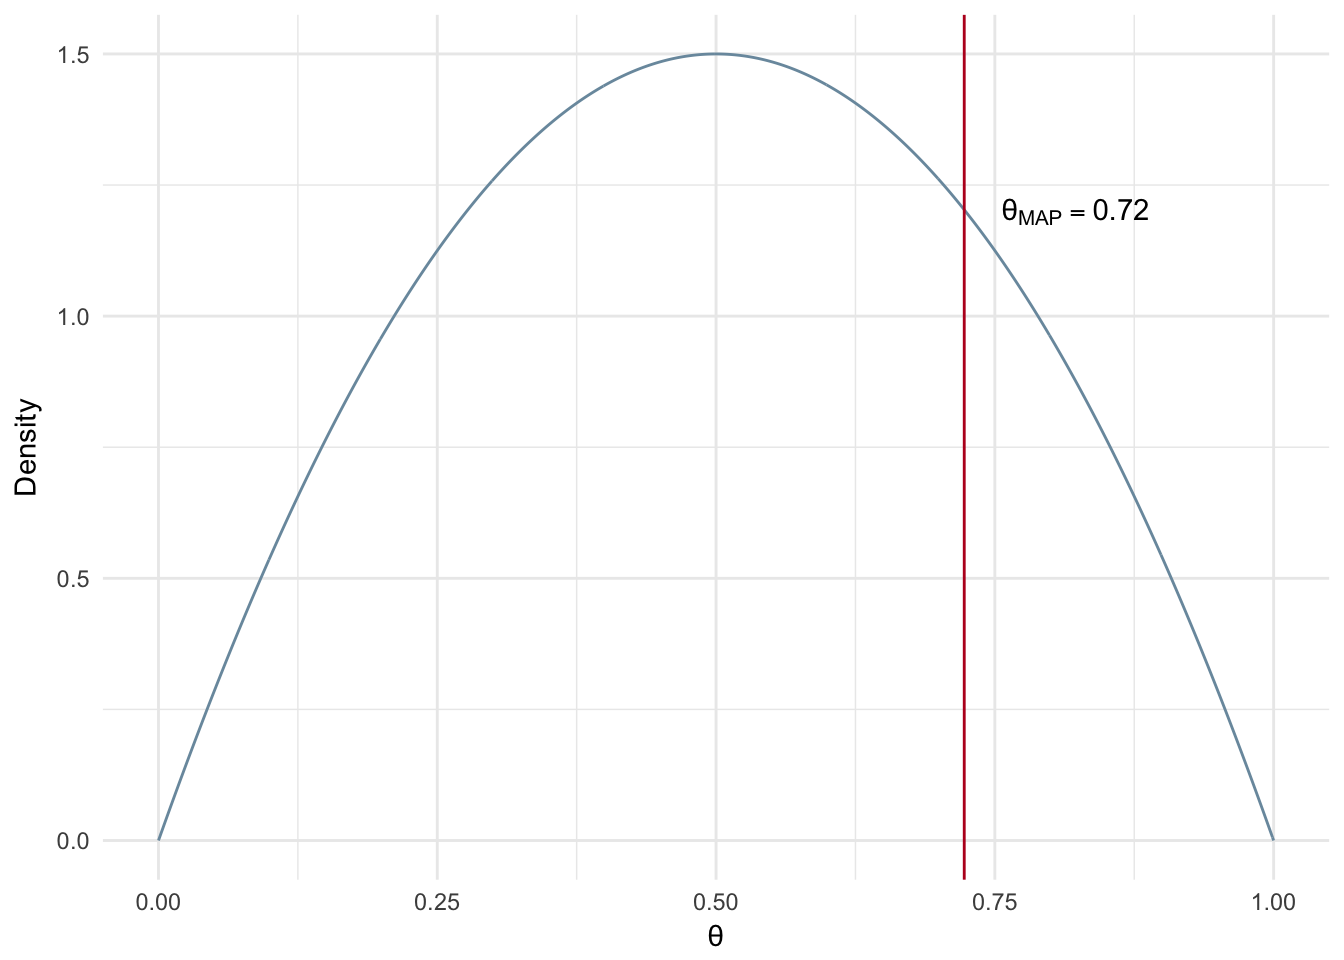
\includegraphics{_main_files/figure-latex/mapLargenUninformedPrior-1.pdf}
\caption{\label{fig:mapLargenUninformedPrior}MAP: Large number of
experiments and uninformed prior}
\end{figure}

\begin{Shaded}
\begin{Highlighting}[]
\NormalTok{n <-}\StringTok{ }\DecValTok{1000}
\NormalTok{heads <-}\StringTok{ }\DecValTok{723}
\NormalTok{tails <-}\StringTok{ }\NormalTok{n}\OperatorTok{-}\NormalTok{heads}


\CommentTok{# ml}
\NormalTok{ml_theta <-}\StringTok{ }\NormalTok{heads}\OperatorTok{/}\NormalTok{n}
\CommentTok{# map}
\NormalTok{B <-}\StringTok{ }\DecValTok{100}
\NormalTok{alpha <-}\StringTok{ }\DecValTok{100}
\NormalTok{possible_theta <-}\StringTok{ }\KeywordTok{seq}\NormalTok{(}\DecValTok{0}\NormalTok{,}\DecValTok{1}\NormalTok{,}\FloatTok{0.001}\NormalTok{)}
\NormalTok{beta_ds <-}\StringTok{ }\KeywordTok{data.frame}\NormalTok{(}\DataTypeTok{theta =}\NormalTok{ possible_theta, }\DataTypeTok{density =} \KeywordTok{dbeta}\NormalTok{(possible_theta, alpha,B))}
\NormalTok{map_theta <-}\StringTok{ }\NormalTok{(heads }\OperatorTok{+}\StringTok{ }\NormalTok{alpha }\OperatorTok{-}\StringTok{ }\DecValTok{1}\NormalTok{)}\OperatorTok{/}\NormalTok{(heads }\OperatorTok{+}\StringTok{ }\NormalTok{tails }\OperatorTok{+}\StringTok{ }\NormalTok{alpha }\OperatorTok{+}\StringTok{ }\NormalTok{B }\OperatorTok{-}\DecValTok{2}\NormalTok{)}
\KeywordTok{ggplot}\NormalTok{(beta_ds, }\KeywordTok{aes}\NormalTok{(}\DataTypeTok{x =}\NormalTok{ theta, }\DataTypeTok{y =}\NormalTok{ density)) }\OperatorTok{+}\StringTok{ }
\StringTok{  }\KeywordTok{geom_line}\NormalTok{(}\DataTypeTok{color=}\StringTok{'#7A99AC'}\NormalTok{) }\OperatorTok{+}\StringTok{ }
\StringTok{  }\KeywordTok{geom_vline}\NormalTok{(}\DataTypeTok{xintercept=}\NormalTok{map_theta, }\DataTypeTok{color =} \StringTok{'#ba0223'}\NormalTok{) }\OperatorTok{+}\StringTok{ }
\StringTok{  }\KeywordTok{annotate}\NormalTok{(}\StringTok{"text"}\NormalTok{, }\DataTypeTok{x =}\NormalTok{ map_theta }\OperatorTok{+}\StringTok{ }\FloatTok{0.1}\NormalTok{, }\DataTypeTok{y=}\FloatTok{1.2}\NormalTok{, }\DataTypeTok{label=} \KeywordTok{paste}\NormalTok{(}\StringTok{"\textbackslash{}U03B8[MAP]=="}\NormalTok{, }\KeywordTok{round}\NormalTok{(map_theta,}\DecValTok{2}\NormalTok{)), }\DataTypeTok{parse=}\NormalTok{T)}\OperatorTok{+}
\StringTok{  }\KeywordTok{labs}\NormalTok{(}\DataTypeTok{x=}\StringTok{'\textbackslash{}U03B8'}\NormalTok{, }\DataTypeTok{y =} \StringTok{'Density'}\NormalTok{) }\OperatorTok{+}\StringTok{ }\KeywordTok{theme_minimal}\NormalTok{()}
\end{Highlighting}
\end{Shaded}

\begin{verbatim}
## Warning in grid.Call(C_stringMetric, as.graphicsAnnot(x$label)): font
## metrics unknown for Unicode character U+03b8

## Warning in grid.Call(C_stringMetric, as.graphicsAnnot(x$label)): font
## metrics unknown for Unicode character U+03b8
\end{verbatim}

\begin{verbatim}
## Warning in grid.Call(C_stringMetric, as.graphicsAnnot(x$label)): conversion
## failure on 'θ' in 'mbcsToSbcs': dot substituted for <ce>
\end{verbatim}

\begin{verbatim}
## Warning in grid.Call(C_stringMetric, as.graphicsAnnot(x$label)): conversion
## failure on 'θ' in 'mbcsToSbcs': dot substituted for <b8>
\end{verbatim}

\begin{verbatim}
## Warning in grid.Call(C_textBounds, as.graphicsAnnot(x$label), x$x, x$y, :
## conversion failure on 'θ' in 'mbcsToSbcs': dot substituted for <ce>
\end{verbatim}

\begin{verbatim}
## Warning in grid.Call(C_textBounds, as.graphicsAnnot(x$label), x$x, x$y, :
## conversion failure on 'θ' in 'mbcsToSbcs': dot substituted for <b8>
\end{verbatim}

\begin{verbatim}
## Warning in grid.Call(C_textBounds, as.graphicsAnnot(x$label), x$x, x$y, :
## conversion failure on 'θ' in 'mbcsToSbcs': dot substituted for <ce>
\end{verbatim}

\begin{verbatim}
## Warning in grid.Call(C_textBounds, as.graphicsAnnot(x$label), x$x, x$y, :
## conversion failure on 'θ' in 'mbcsToSbcs': dot substituted for <b8>
\end{verbatim}

\begin{verbatim}
## Warning in grid.Call(C_textBounds, as.graphicsAnnot(x$label), x$x, x$y, :
## conversion failure on 'θ' in 'mbcsToSbcs': dot substituted for <ce>
\end{verbatim}

\begin{verbatim}
## Warning in grid.Call(C_textBounds, as.graphicsAnnot(x$label), x$x, x$y, :
## conversion failure on 'θ' in 'mbcsToSbcs': dot substituted for <b8>
\end{verbatim}

\begin{verbatim}
## Warning in grid.Call(C_textBounds, as.graphicsAnnot(x$label), x$x, x$y, :
## conversion failure on 'θ' in 'mbcsToSbcs': dot substituted for <ce>
\end{verbatim}

\begin{verbatim}
## Warning in grid.Call(C_textBounds, as.graphicsAnnot(x$label), x$x, x$y, :
## conversion failure on 'θ' in 'mbcsToSbcs': dot substituted for <b8>
\end{verbatim}

\begin{verbatim}
## Warning in grid.Call(C_textBounds, as.graphicsAnnot(x$label), x$x, x$y, :
## conversion failure on 'θ' in 'mbcsToSbcs': dot substituted for <ce>
\end{verbatim}

\begin{verbatim}
## Warning in grid.Call(C_textBounds, as.graphicsAnnot(x$label), x$x, x$y, :
## conversion failure on 'θ' in 'mbcsToSbcs': dot substituted for <b8>
\end{verbatim}

\begin{verbatim}
## Warning in grid.Call.graphics(C_text, as.graphicsAnnot(x$label), x$x, x
## $y, : font metrics unknown for Unicode character U+03b8

## Warning in grid.Call.graphics(C_text, as.graphicsAnnot(x$label), x$x, x
## $y, : font metrics unknown for Unicode character U+03b8
\end{verbatim}

\begin{verbatim}
## Warning in grid.Call.graphics(C_text, as.graphicsAnnot(x$label), x$x, x
## $y, : conversion failure on 'θ' in 'mbcsToSbcs': dot substituted for <ce>
\end{verbatim}

\begin{verbatim}
## Warning in grid.Call.graphics(C_text, as.graphicsAnnot(x$label), x$x, x
## $y, : conversion failure on 'θ' in 'mbcsToSbcs': dot substituted for <b8>
\end{verbatim}

\begin{verbatim}
## Warning in grid.Call(C_textBounds, as.graphicsAnnot(x$label), x$x, x$y, :
## conversion failure on 'θ' in 'mbcsToSbcs': dot substituted for <ce>
\end{verbatim}

\begin{verbatim}
## Warning in grid.Call(C_textBounds, as.graphicsAnnot(x$label), x$x, x$y, :
## conversion failure on 'θ' in 'mbcsToSbcs': dot substituted for <b8>
\end{verbatim}

\begin{verbatim}
## Warning in grid.Call(C_textBounds, as.graphicsAnnot(x$label), x$x, x$y, :
## conversion failure on 'θ' in 'mbcsToSbcs': dot substituted for <ce>
\end{verbatim}

\begin{verbatim}
## Warning in grid.Call(C_textBounds, as.graphicsAnnot(x$label), x$x, x$y, :
## conversion failure on 'θ' in 'mbcsToSbcs': dot substituted for <b8>
\end{verbatim}

\begin{verbatim}
## Warning in grid.Call.graphics(C_text, as.graphicsAnnot(x$label), x$x, x
## $y, : conversion failure on 'θ' in 'mbcsToSbcs': dot substituted for <ce>
\end{verbatim}

\begin{verbatim}
## Warning in grid.Call.graphics(C_text, as.graphicsAnnot(x$label), x$x, x
## $y, : conversion failure on 'θ' in 'mbcsToSbcs': dot substituted for <b8>
\end{verbatim}

\begin{figure}
\centering
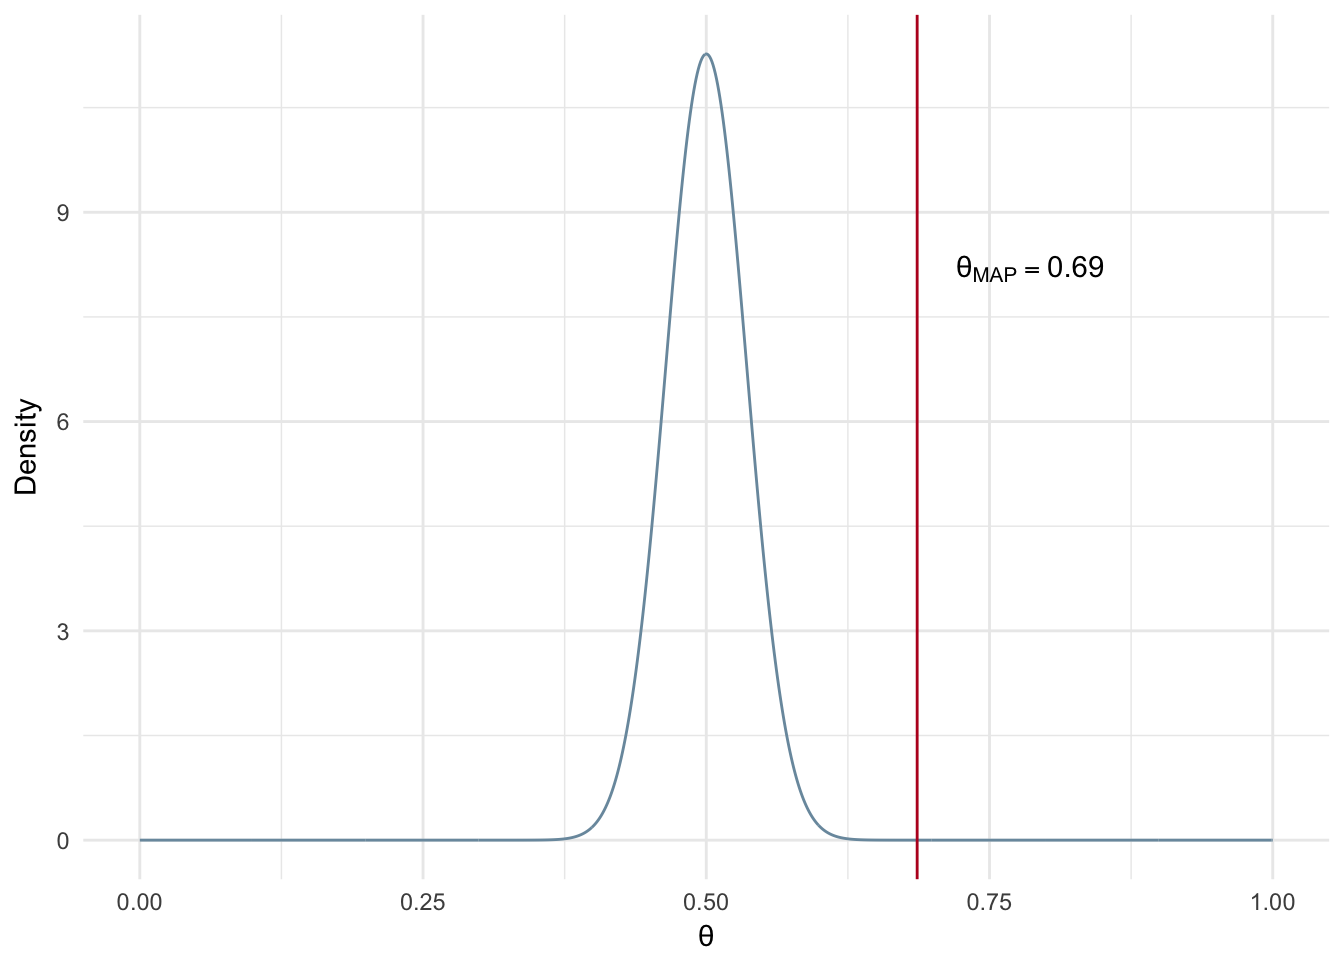
\includegraphics{_main_files/figure-latex/mapLargeInformedPrior-1.pdf}
\caption{\label{fig:mapLargeInformedPrior}MAP: Large number of experiments
and informed prior}
\end{figure}

\section{Bayesian Inference}\label{bayesian-inference}

Where does the evidence term go?

Make an example of this and cite Krutchke - I assume in the earlier
chapters there is something present.

For explanation \#1 you can use the metropolis hastings algorithm
examples. You are sampling from a posterior without a normalizing
factor, but you use the proportions of the samples to determine the
probability (i.e.~you infer the normalization term through sampling - it
is basically built in at that point.) {[}Explanation 1: The normalizing
constant is not interesting, this is very common in bayesian statistics,
. With Gibbs sampling, Metropolis-Hasting or any other Monte Carlo
method, what you are doing is drawing samples from this posterior. That
is, the more density around a point, the more samples you'll get there.

Then, once you have enough samples from this posterior distribution, you
know that the normalized density at some point xx is the proportion of
samples that felt at that point.

You can even plot an histogram on the samples to see the (unnormalized)
posterior.

In other words, if I give you the samples
1,3,4,5,1\ldots{}..,3,4,16,11,3,4,5,1\ldots{}..,3,4,16,1 and I tell you
these are samples from a density function, you know to compute the
probability of every value.

\ldots{}.. Explanation 3 If you use conjugate priors for the individual
variables, the denominator of their conditional probability will be
always nice and familiar, and you will know what the normalizing
constant in the denominator is. This is why Gibbs sampling is so popular
when the joint probability is ugly but the conditional probabilities are
nice.{]}(\url{https://stats.stackexchange.com/questions/138644/confusion-in-gibbs-sampling\#138648})

For explanation \#3 use the coin flip example\ldots{} p(theta1,
theta2\textbar{}D) show how denominator p(d) drops out.

\subsection{Conjugate Priors}\label{conjugate-priors}

The general premise of conjugate priors is that the prior has the same
form as the posterior distribution. Ok, but what does that mean for us?
In a pragmatic sense it means we need to look for a \textbf{pattern}
when solving for our posterior.

\textbf{PATTERN MATCHING}

Let's take the coin flip example. We want to estimate the posterior, the
probability of \(\theta\) given the observed data. Obviously we don't
have observed data so we will need to use the likelihood and the prior
to estimate the posterior. For this case we will use the beta
distribution to estimate the prior with the form:

{[}BETA DISTRIBUTION - use overbraces to show the pattern {]}

\subsubsection{Bernoulli \& Beta}\label{bernoulli-beta}

The beta distribution serves as the conjugate prior for the bernoulli
distribution.

Putting the conjugate prior to use\ldots{}.estimating the posterior

\[
\underbrace{p(\theta|D)}_{posterior} = {\overbrace{p(D|\theta)}^{likelihood}
  \overbrace{p(\theta)}^{prior} \over \underbrace{p(D)}_{evidence}}
\tag{15}
\] When estimating the posterior, the evidence term is dropped
out\ldots{}scaling factor, blah blah

\[
\underbrace{p(\theta|D)}_{posterior}  \propto  {\overbrace{p(D|\theta)}^{likelihood}
  \overbrace{p(\theta)}^{prior}}
\tag{16}
\] To estimate the posterior of the bernoulli distribution \[
p(\theta|z,N) \propto \overbrace{\theta^z(1-\theta)^{(N-z)}}^{likelihood} \overbrace{{\theta^{(a-1)}(1-\theta)^{(b-1)}}\over \beta(a,b)}^{prior}
\tag{17}
\] After combining terms we get\ldots{}. \[
p(\theta|z,N) \propto \overbrace{\theta^{(a + z -1)}(1-\theta)^{(N-z+b-1)}}^{Same \hspace{1 mm} Pattern \hspace{1 mm} as \hspace{1 mm} Likelihood}
\tag{18}
\]

\subsection{Gibbs Sampling}\label{gibbs-sampling}

This should include a drawing of sampling from two different jars At
each iteration the jar is changed (the parameters of the distribution)

Mathematical representation of what happens in Gibbs Sampling:

\[
\begin{aligned}
&p(\theta_{1}^{i+1}) \sim p(\theta_{1}^{i}|\theta_{2}^{i}, \theta_{3}^{i},..., \theta{n}^{i}) \\
&p(\theta_{2}^{i+1}) \sim p(\theta_{2}^{i}|\theta_{1}^{i+1}, \theta_{3}^{i},..., \theta{n}^{i}) \\
&p(\theta_{3}^{i+1}) \sim p(\theta_{3}^{i}|\theta_{1}^{i+1}, \theta_{2}^{i+1},..., \theta{n}^{i}) \\
&................................ \\ 
&p(\theta_{n}^{i+1}) \sim p(\theta_{n}^{i}|\theta_{1}^{i+1}, \theta_{2}^{i+1},..., \theta_{n-1}^{i+1}) \\
\end{aligned}
\tag{19}
\]

\subsection{Bias of Two Coins}\label{bias-of-two-coins}

Code example of 2 coins

\begin{Shaded}
\begin{Highlighting}[]
\NormalTok{a =}\StringTok{ }\DecValTok{2}
\NormalTok{b =}\StringTok{ }\DecValTok{2}

\NormalTok{z1 =}\StringTok{ }\DecValTok{11}
\NormalTok{N1 =}\StringTok{ }\DecValTok{14}
\NormalTok{z2 =}\StringTok{ }\DecValTok{7}
\NormalTok{N2 =}\StringTok{ }\DecValTok{14}


\NormalTok{theta =}\StringTok{ }\KeywordTok{rep}\NormalTok{(}\FloatTok{0.5}\NormalTok{,}\DecValTok{2}\NormalTok{)}
\NormalTok{niters =}\StringTok{ }\DecValTok{10000}
\NormalTok{burnin =}\StringTok{ }\DecValTok{500}

\NormalTok{thetas =}\StringTok{ }\KeywordTok{matrix}\NormalTok{(}\DecValTok{0}\NormalTok{, }\DataTypeTok{nrow =}\NormalTok{ (niters}\OperatorTok{-}\NormalTok{burnin), }\DataTypeTok{ncol=}\DecValTok{2}\NormalTok{)}
\ControlFlowTok{for}\NormalTok{ (i }\ControlFlowTok{in} \DecValTok{1}\OperatorTok{:}\NormalTok{niters)\{}

\NormalTok{  theta1 =}\StringTok{ }\KeywordTok{rbeta}\NormalTok{(}\DataTypeTok{n =} \DecValTok{1}\NormalTok{, }\DataTypeTok{shape1 =}\NormalTok{ a }\OperatorTok{+}\StringTok{ }\NormalTok{z1, }\DataTypeTok{shape2 =}\NormalTok{ b }\OperatorTok{+}\StringTok{ }\NormalTok{N1 }\OperatorTok{-}\StringTok{ }\NormalTok{z1)}
  \CommentTok{# get value theta2| all other vars}
\NormalTok{  theta2 =}\StringTok{ }\KeywordTok{rbeta}\NormalTok{(}\DataTypeTok{n =} \DecValTok{1}\NormalTok{, }\DataTypeTok{shape1 =}\NormalTok{ a }\OperatorTok{+}\StringTok{ }\NormalTok{z2, }\DataTypeTok{shape2 =}\NormalTok{b }\OperatorTok{+}\StringTok{ }\NormalTok{N2 }\OperatorTok{-}\StringTok{ }\NormalTok{z2)}
  
  \ControlFlowTok{if}\NormalTok{ (i }\OperatorTok{>=}\StringTok{ }\NormalTok{burnin)\{}
\NormalTok{    thetas[(i}\OperatorTok{-}\NormalTok{burnin), ] =}\StringTok{ }\KeywordTok{c}\NormalTok{(theta1, theta2)}
\NormalTok{  \}}
\NormalTok{\}}


\NormalTok{ds <-}\StringTok{ }\KeywordTok{data.frame}\NormalTok{(}\DataTypeTok{theta1 =}\NormalTok{ thetas[,}\DecValTok{1}\NormalTok{], }\DataTypeTok{theta2=}\NormalTok{ thetas[,}\DecValTok{2}\NormalTok{])}
\KeywordTok{ggplot}\NormalTok{(ds, }\KeywordTok{aes}\NormalTok{(}\DataTypeTok{x=}\NormalTok{theta1)) }\OperatorTok{+}\StringTok{ }\KeywordTok{geom_histogram}\NormalTok{(}\KeywordTok{aes}\NormalTok{(}\DataTypeTok{y=}\NormalTok{..density..),}\DataTypeTok{color=}\StringTok{'#1A384A'}\NormalTok{, }\DataTypeTok{fill=}\StringTok{'#7A99AC'}\NormalTok{) }\OperatorTok{+}\StringTok{ }
\StringTok{  }\KeywordTok{labs}\NormalTok{(}\DataTypeTok{title =} \KeywordTok{expression}\NormalTok{(theta[}\DecValTok{1}\NormalTok{]}\OperatorTok{~}\NormalTok{Estimate), }\DataTypeTok{x=}\KeywordTok{expression}\NormalTok{(theta[}\DecValTok{1}\NormalTok{]), }\DataTypeTok{y =} \StringTok{'Density'}\NormalTok{) }\OperatorTok{+}\StringTok{ }
\StringTok{  }\KeywordTok{geom_vline}\NormalTok{(}\DataTypeTok{xintercept =} \KeywordTok{mean}\NormalTok{(ds}\OperatorTok{$}\NormalTok{theta1), }\DataTypeTok{color=}\StringTok{'#b7091a'}\NormalTok{) }\OperatorTok{+}
\StringTok{  }\KeywordTok{theme_minimal}\NormalTok{()}
\end{Highlighting}
\end{Shaded}

\begin{figure}
\centering
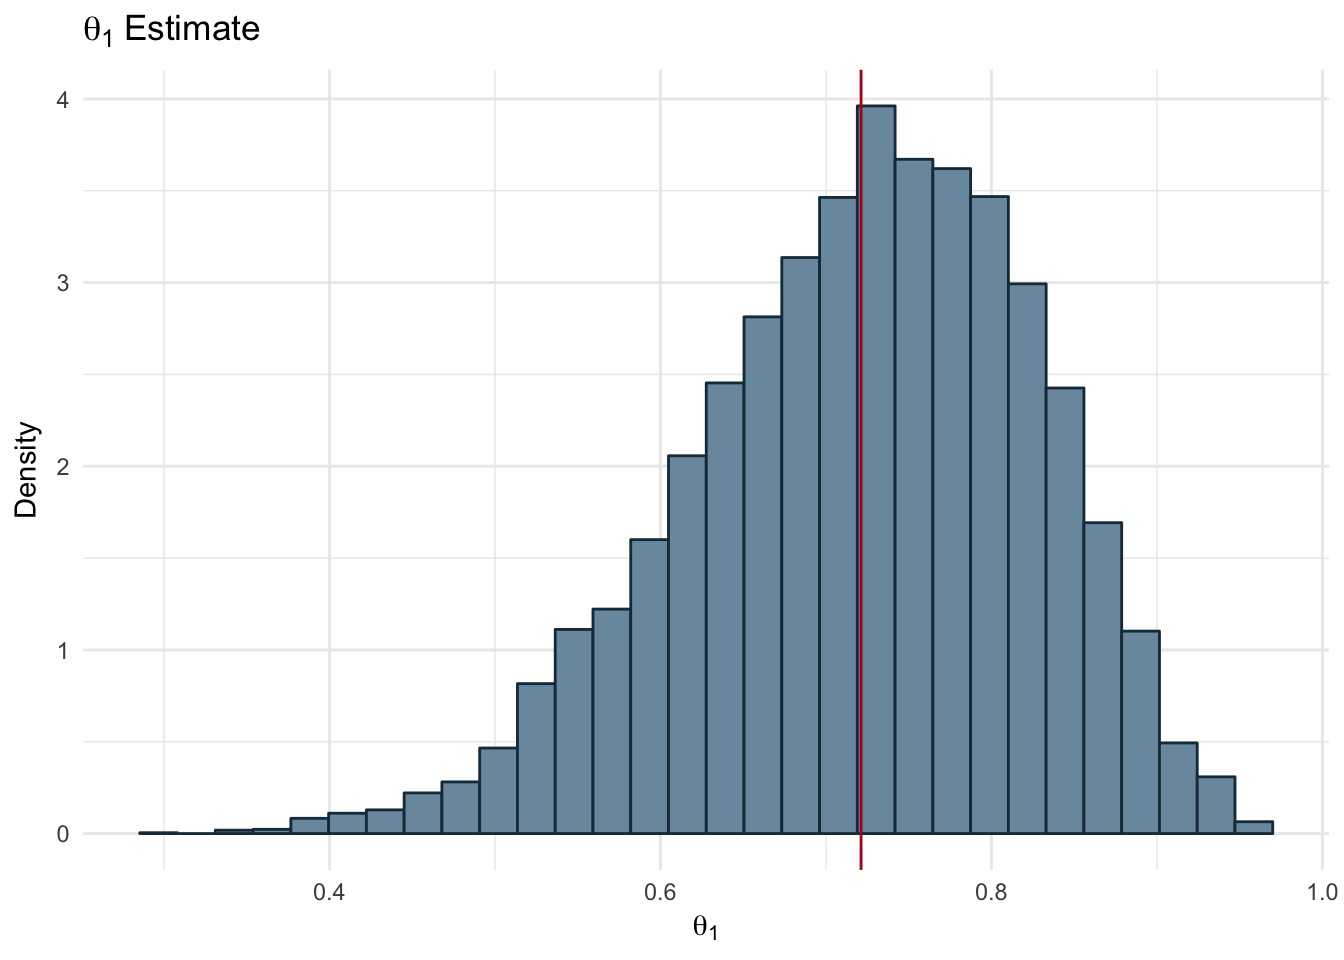
\includegraphics{_main_files/figure-latex/2coins-1.pdf}
\caption{\label{fig:2coins}Bias of Two Coins: Theta 1}
\end{figure}

\begin{Shaded}
\begin{Highlighting}[]
\KeywordTok{ggplot}\NormalTok{(ds, }\KeywordTok{aes}\NormalTok{(}\DataTypeTok{x=}\NormalTok{theta2)) }\OperatorTok{+}\StringTok{ }\KeywordTok{geom_histogram}\NormalTok{(}\KeywordTok{aes}\NormalTok{(}\DataTypeTok{y=}\NormalTok{..density..),}\DataTypeTok{color=}\StringTok{'#1A384A'}\NormalTok{, }\DataTypeTok{fill=}\StringTok{'#7A99AC'}\NormalTok{) }\OperatorTok{+}\StringTok{ }
\StringTok{  }\KeywordTok{labs}\NormalTok{(}\DataTypeTok{title =} \KeywordTok{expression}\NormalTok{(theta[}\DecValTok{2}\NormalTok{]}\OperatorTok{~}\NormalTok{Estimate), }\DataTypeTok{x=}\KeywordTok{expression}\NormalTok{(theta[}\DecValTok{2}\NormalTok{]), }\DataTypeTok{y =} \StringTok{'Density'}\NormalTok{) }\OperatorTok{+}\StringTok{ }
\StringTok{  }\KeywordTok{geom_vline}\NormalTok{(}\DataTypeTok{xintercept =} \KeywordTok{mean}\NormalTok{(ds}\OperatorTok{$}\NormalTok{theta2), }\DataTypeTok{color=}\StringTok{'#b7091a'}\NormalTok{) }\OperatorTok{+}\StringTok{ }
\StringTok{  }\KeywordTok{theme_minimal}\NormalTok{()}
\end{Highlighting}
\end{Shaded}

\begin{figure}
\centering
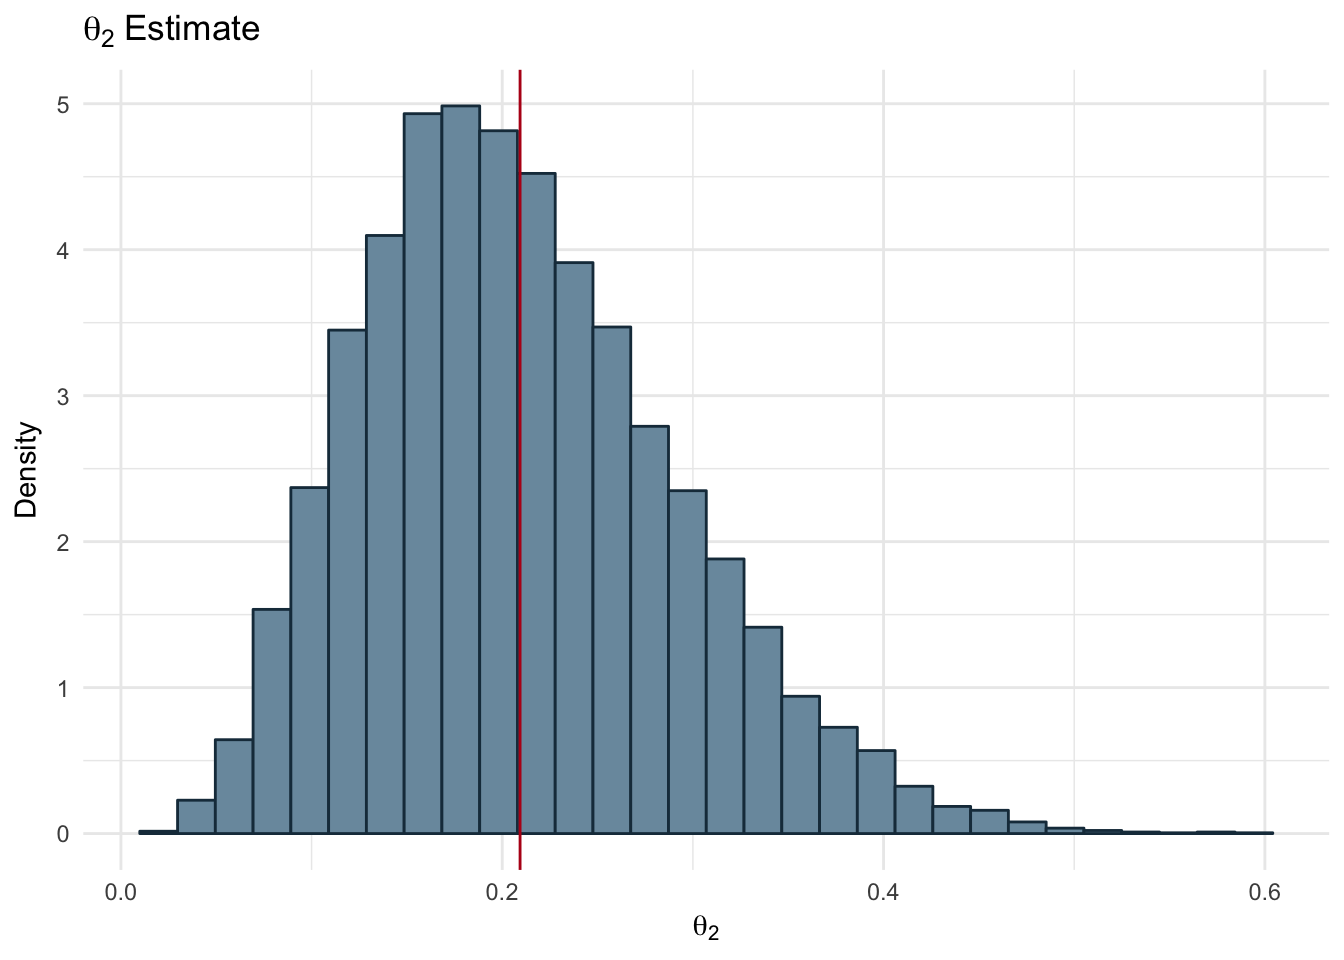
\includegraphics{_main_files/figure-latex/2coins2-1.pdf}
\caption{\label{fig:2coins2}Bias of Two Coins - Theta 2}
\end{figure}

\subsection{Change Point Example}\label{change-point-example}

What if the problem we are solving is more complicated. Let's say I flip
a coin repeatedly, but at some point I switch to another coin with a
different bias (\(\theta\)). I want to detect the point in time when
coin 1 was swapped out for coin 2.

IMAGE PLACE HOLDER - MAKE A DRAWING OF FLIPPING TWO COINS ON A TIME
SCALE

\begin{Shaded}
\begin{Highlighting}[]
\NormalTok{real_thetas <-}\StringTok{ }\KeywordTok{c}\NormalTok{(}\FloatTok{0.2}\NormalTok{, }\FloatTok{0.6}\NormalTok{)}
\NormalTok{N <-}\StringTok{ }\DecValTok{300}
\NormalTok{a =}\StringTok{ }\DecValTok{2}
\NormalTok{b =}\StringTok{ }\DecValTok{3}
\NormalTok{change_point <-}\StringTok{ }\DecValTok{100}
\NormalTok{x <-}\StringTok{ }\KeywordTok{c}\NormalTok{(}\KeywordTok{rbinom}\NormalTok{(}\DecValTok{1}\OperatorTok{:}\NormalTok{change_point, }\DecValTok{1}\NormalTok{, real_thetas[}\DecValTok{1}\NormalTok{]),}\KeywordTok{rbinom}\NormalTok{((change_point}\OperatorTok{+}\DecValTok{1}\NormalTok{)}\OperatorTok{:}\NormalTok{N, }\DecValTok{1}\NormalTok{, real_thetas[}\DecValTok{2}\NormalTok{]))}


\NormalTok{## Initialize all parameters}

\CommentTok{# n ~ uniform }
\NormalTok{n <-}\StringTok{ }\KeywordTok{round}\NormalTok{(N}\OperatorTok{*}\KeywordTok{runif}\NormalTok{(}\DecValTok{1}\NormalTok{))}
\CommentTok{# theta1 ~ beta(a,b)}
\NormalTok{theta1 <-}\StringTok{ }\KeywordTok{rbeta}\NormalTok{(}\DecValTok{1}\NormalTok{, a, b)}
\CommentTok{# theta2 ~ beta(a,b)}
\NormalTok{theta2 <-}\StringTok{ }\KeywordTok{rbeta}\NormalTok{(}\DecValTok{1}\NormalTok{, a, b)}



\NormalTok{niters =}\StringTok{ }\DecValTok{10000}
\NormalTok{burnin =}\StringTok{ }\DecValTok{2000}
\CommentTok{# sigma = np.diag([0.2,0.2])}

\CommentTok{# thetas = np.zeros((niters-burnin,2), np.float)}
\NormalTok{params =}\StringTok{ }\KeywordTok{matrix}\NormalTok{(}\DecValTok{0}\NormalTok{, }\DataTypeTok{nrow =}\NormalTok{ (niters}\OperatorTok{-}\NormalTok{burnin), }\DataTypeTok{ncol=}\DecValTok{3}\NormalTok{)}
\ControlFlowTok{for}\NormalTok{ (i }\ControlFlowTok{in} \DecValTok{1}\OperatorTok{:}\NormalTok{niters)\{}
  
  
\NormalTok{  z1 <-}\StringTok{ }\KeywordTok{sum}\NormalTok{(x[}\DecValTok{1}\OperatorTok{:}\NormalTok{n])}
  \ControlFlowTok{if}\NormalTok{(n }\OperatorTok{==}\StringTok{ }\NormalTok{N)\{}
\NormalTok{    z2 <-}\StringTok{ }\DecValTok{0}
\NormalTok{  \}}\ControlFlowTok{else}\NormalTok{\{}
\NormalTok{    z2 <-}\StringTok{ }\KeywordTok{sum}\NormalTok{(x[(n}\OperatorTok{+}\DecValTok{1}\NormalTok{)}\OperatorTok{:}\NormalTok{N])}
\NormalTok{  \}}
\NormalTok{  theta1 =}\StringTok{ }\KeywordTok{rbeta}\NormalTok{(}\DataTypeTok{n =} \DecValTok{1}\NormalTok{, }\DataTypeTok{shape1 =}\NormalTok{ a }\OperatorTok{+}\StringTok{ }\NormalTok{z1, }\DataTypeTok{shape2 =}\NormalTok{ b }\OperatorTok{+}\StringTok{ }\NormalTok{n }\OperatorTok{-}\StringTok{ }\NormalTok{z1)}
  \CommentTok{# get value theta2| all other vars}
\NormalTok{  theta2 =}\StringTok{ }\KeywordTok{rbeta}\NormalTok{(}\DataTypeTok{n =} \DecValTok{1}\NormalTok{, }\DataTypeTok{shape1 =}\NormalTok{ a }\OperatorTok{+}\StringTok{ }\NormalTok{z2, }\DataTypeTok{shape2 =}\NormalTok{N}\OperatorTok{-}\NormalTok{n}\OperatorTok{-}\DecValTok{1}\OperatorTok{-}\NormalTok{z2}\OperatorTok{+}\NormalTok{b)}
  
  
\NormalTok{  ## 2 things: 1 - should I be summing all the values over these? }
  \CommentTok{# No - the product is being calculated due to the sum - should be fine}
\NormalTok{  n_multi <-}\StringTok{ }\KeywordTok{rep}\NormalTok{(}\DecValTok{0}\NormalTok{, N)}
  \ControlFlowTok{for}\NormalTok{(steps }\ControlFlowTok{in} \DecValTok{1}\OperatorTok{:}\NormalTok{N)\{}
    \ControlFlowTok{if}\NormalTok{(steps}\OperatorTok{==}\NormalTok{N }\OperatorTok{||}\StringTok{ }\NormalTok{theta2 }\OperatorTok{==}\StringTok{ }\DecValTok{1}\NormalTok{)\{}
\NormalTok{      n_multi[steps] <-}\StringTok{ }\KeywordTok{log}\NormalTok{(theta1}\OperatorTok{^}\KeywordTok{sum}\NormalTok{(x[}\DecValTok{1}\OperatorTok{:}\NormalTok{steps]) }\OperatorTok{*}\StringTok{ }\NormalTok{(}\DecValTok{1}\OperatorTok{-}\NormalTok{theta1)}\OperatorTok{^}\NormalTok{(steps}\OperatorTok{-}\KeywordTok{sum}\NormalTok{(x[}\DecValTok{1}\OperatorTok{:}\NormalTok{steps])))}
\NormalTok{    \}}\ControlFlowTok{else}\NormalTok{\{}
\NormalTok{      n_multi[steps] <-}\StringTok{ }\KeywordTok{log}\NormalTok{(theta1}\OperatorTok{^}\KeywordTok{sum}\NormalTok{(x[}\DecValTok{1}\OperatorTok{:}\NormalTok{steps]) }\OperatorTok{*}\StringTok{ }\NormalTok{(}\DecValTok{1}\OperatorTok{-}\NormalTok{theta1)}\OperatorTok{^}\NormalTok{(steps}\OperatorTok{-}\KeywordTok{sum}\NormalTok{(x[}\DecValTok{1}\OperatorTok{:}\NormalTok{steps]))) }\OperatorTok{+}
\StringTok{        }\KeywordTok{log}\NormalTok{(theta2}\OperatorTok{^}\KeywordTok{sum}\NormalTok{(x[(steps }\OperatorTok{+}\StringTok{ }\DecValTok{1}\NormalTok{)}\OperatorTok{:}\NormalTok{N]) }\OperatorTok{*}\StringTok{ }\NormalTok{(}\DecValTok{1}\OperatorTok{-}\NormalTok{theta2)}\OperatorTok{^}\NormalTok{(N}\OperatorTok{-}\NormalTok{steps}\OperatorTok{-}\DecValTok{1}\OperatorTok{-}\KeywordTok{sum}\NormalTok{(x[(steps}\OperatorTok{+}\DecValTok{1}\NormalTok{)}\OperatorTok{:}\NormalTok{N])))}
\NormalTok{    \}}
\NormalTok{  \}}
  
\NormalTok{  n_multi <-}\StringTok{ }\KeywordTok{exp}\NormalTok{(n_multi }\OperatorTok{-}\StringTok{ }\KeywordTok{max}\NormalTok{(n_multi))}
  \CommentTok{# what about for n? }
\NormalTok{  n <-}\StringTok{ }\KeywordTok{which}\NormalTok{(}\KeywordTok{rmultinom}\NormalTok{(}\DecValTok{1}\NormalTok{, }\DecValTok{1}\NormalTok{, n_multi}\OperatorTok{/}\KeywordTok{sum}\NormalTok{(n_multi))[,}\DecValTok{1}\NormalTok{] }\OperatorTok{==}\DecValTok{1}\NormalTok{)}
  \ControlFlowTok{if}\NormalTok{ (i }\OperatorTok{>=}\StringTok{ }\NormalTok{burnin)\{}
\NormalTok{    params[(i}\OperatorTok{-}\NormalTok{burnin), ] =}\StringTok{ }\KeywordTok{c}\NormalTok{(theta1,theta2, n)}
\NormalTok{  \}}
\NormalTok{\}}

\NormalTok{ds <-}\StringTok{ }\KeywordTok{data.frame}\NormalTok{(}\DataTypeTok{x =}\NormalTok{ x, }\DataTypeTok{theta =} \KeywordTok{c}\NormalTok{(}\KeywordTok{rep}\NormalTok{(real_thetas[}\DecValTok{1}\NormalTok{],N}\OperatorTok{-}\NormalTok{change_point),}
                                  \KeywordTok{rep}\NormalTok{(real_thetas[}\DecValTok{2}\NormalTok{],change_point)), }
                 \DataTypeTok{sample_index =} \KeywordTok{seq}\NormalTok{(}\DecValTok{1}\OperatorTok{:}\KeywordTok{length}\NormalTok{(x)))}
\end{Highlighting}
\end{Shaded}

\begin{Shaded}
\begin{Highlighting}[]
\NormalTok{params_df <-}\StringTok{ }\KeywordTok{as.data.frame}\NormalTok{(params)}
\KeywordTok{names}\NormalTok{(params_df) <-}\StringTok{ }\KeywordTok{c}\NormalTok{(}\StringTok{'theta1'}\NormalTok{, }\StringTok{'theta2'}\NormalTok{, }\StringTok{'change_point'}\NormalTok{)}

\KeywordTok{ggplot}\NormalTok{(params_df, }\KeywordTok{aes}\NormalTok{(}\DataTypeTok{x =}\NormalTok{ change_point)) }\OperatorTok{+}\StringTok{ }
\StringTok{  }\KeywordTok{geom_histogram}\NormalTok{(}\DataTypeTok{fill=}\StringTok{"#7A99AC"}\NormalTok{, }\DataTypeTok{color =}\StringTok{'#1A384A'}\NormalTok{) }\OperatorTok{+}
\StringTok{  }\KeywordTok{theme_minimal}\NormalTok{() }\OperatorTok{+}\StringTok{ }
\StringTok{  }\KeywordTok{geom_vline}\NormalTok{(}\DataTypeTok{xintercept =} \KeywordTok{mean}\NormalTok{(params_df}\OperatorTok{$}\NormalTok{change_point), }\DataTypeTok{color=}\StringTok{'#b7091a'}\NormalTok{) }\OperatorTok{+}
\StringTok{  }\KeywordTok{labs}\NormalTok{(}\DataTypeTok{title =} \StringTok{'Change Point Estimate'}\NormalTok{, }\DataTypeTok{x=}\StringTok{'Change Point'}\NormalTok{, }\DataTypeTok{y =} \StringTok{'Density'}\NormalTok{) }
\end{Highlighting}
\end{Shaded}

\begin{figure}
\centering
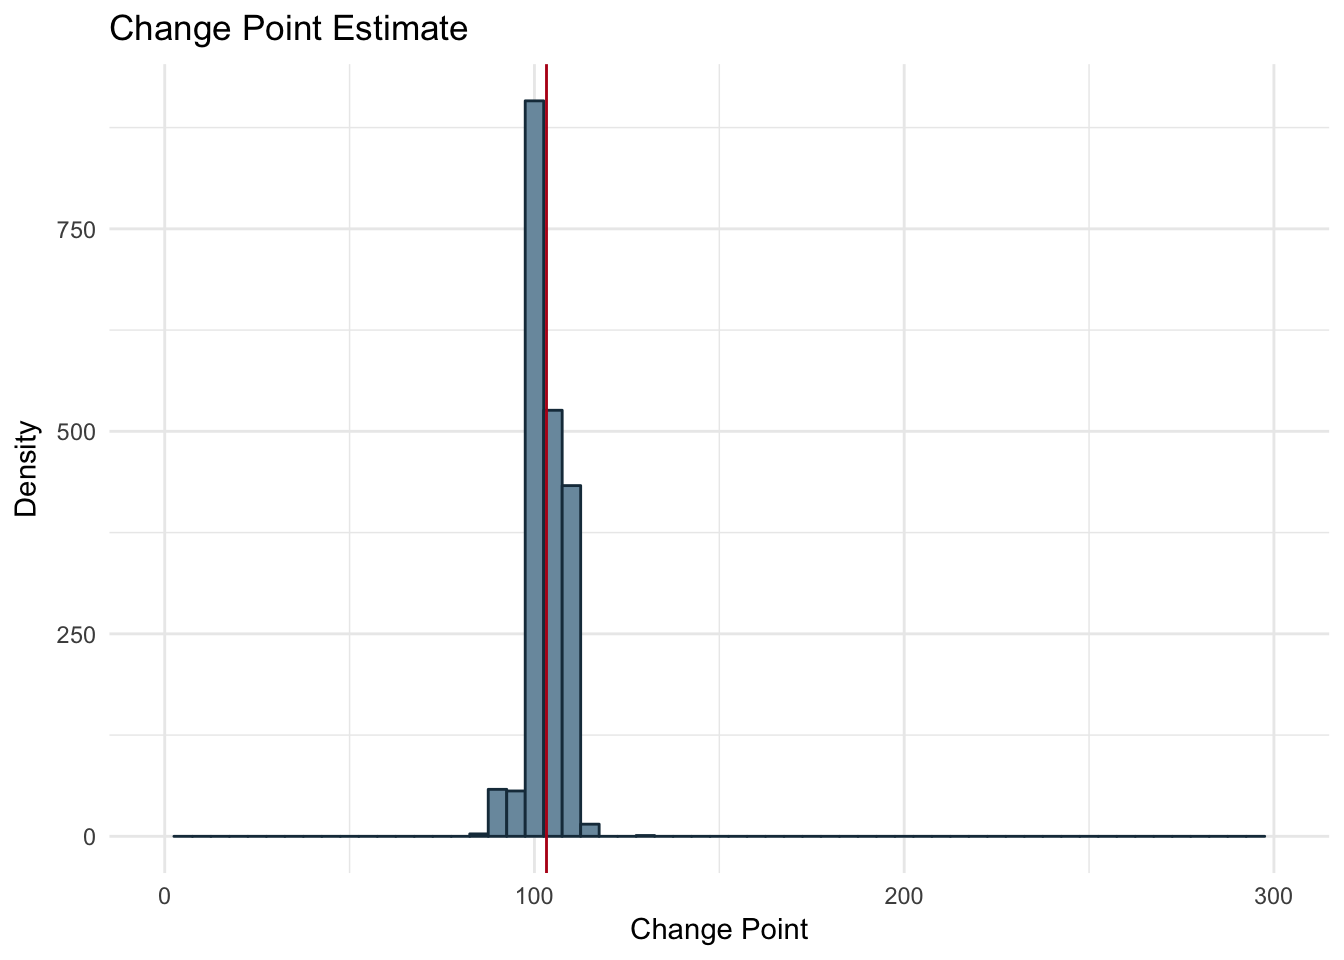
\includegraphics{_main_files/figure-latex/bernChangePointN-1.pdf}
\caption{\label{fig:bernChangePointN}Estimated Change Point}
\end{figure}

\begin{Shaded}
\begin{Highlighting}[]
\KeywordTok{ggplot}\NormalTok{(params_df, }\KeywordTok{aes}\NormalTok{(}\DataTypeTok{x =}\NormalTok{ theta1)) }\OperatorTok{+}\StringTok{ }
\StringTok{  }\KeywordTok{geom_histogram}\NormalTok{(}\DataTypeTok{fill=}\StringTok{"#7A99AC"}\NormalTok{, }\DataTypeTok{color =}\StringTok{'#1A384A'}\NormalTok{ ) }\OperatorTok{+}\StringTok{ }
\StringTok{  }\KeywordTok{theme_minimal}\NormalTok{() }\OperatorTok{+}\StringTok{ }
\StringTok{  }\KeywordTok{geom_vline}\NormalTok{(}\DataTypeTok{xintercept =} \KeywordTok{mean}\NormalTok{(params_df}\OperatorTok{$}\NormalTok{theta1), }\DataTypeTok{color=}\StringTok{'#b7091a'}\NormalTok{) }\OperatorTok{+}
\StringTok{  }\KeywordTok{labs}\NormalTok{(}\DataTypeTok{title =} \KeywordTok{expression}\NormalTok{(theta[}\DecValTok{1}\NormalTok{]}\OperatorTok{~}\NormalTok{Estimate), }\DataTypeTok{x=}\KeywordTok{expression}\NormalTok{(theta[}\DecValTok{1}\NormalTok{]), }\DataTypeTok{y =} \StringTok{'Density'}\NormalTok{) }
\end{Highlighting}
\end{Shaded}

\begin{figure}
\centering
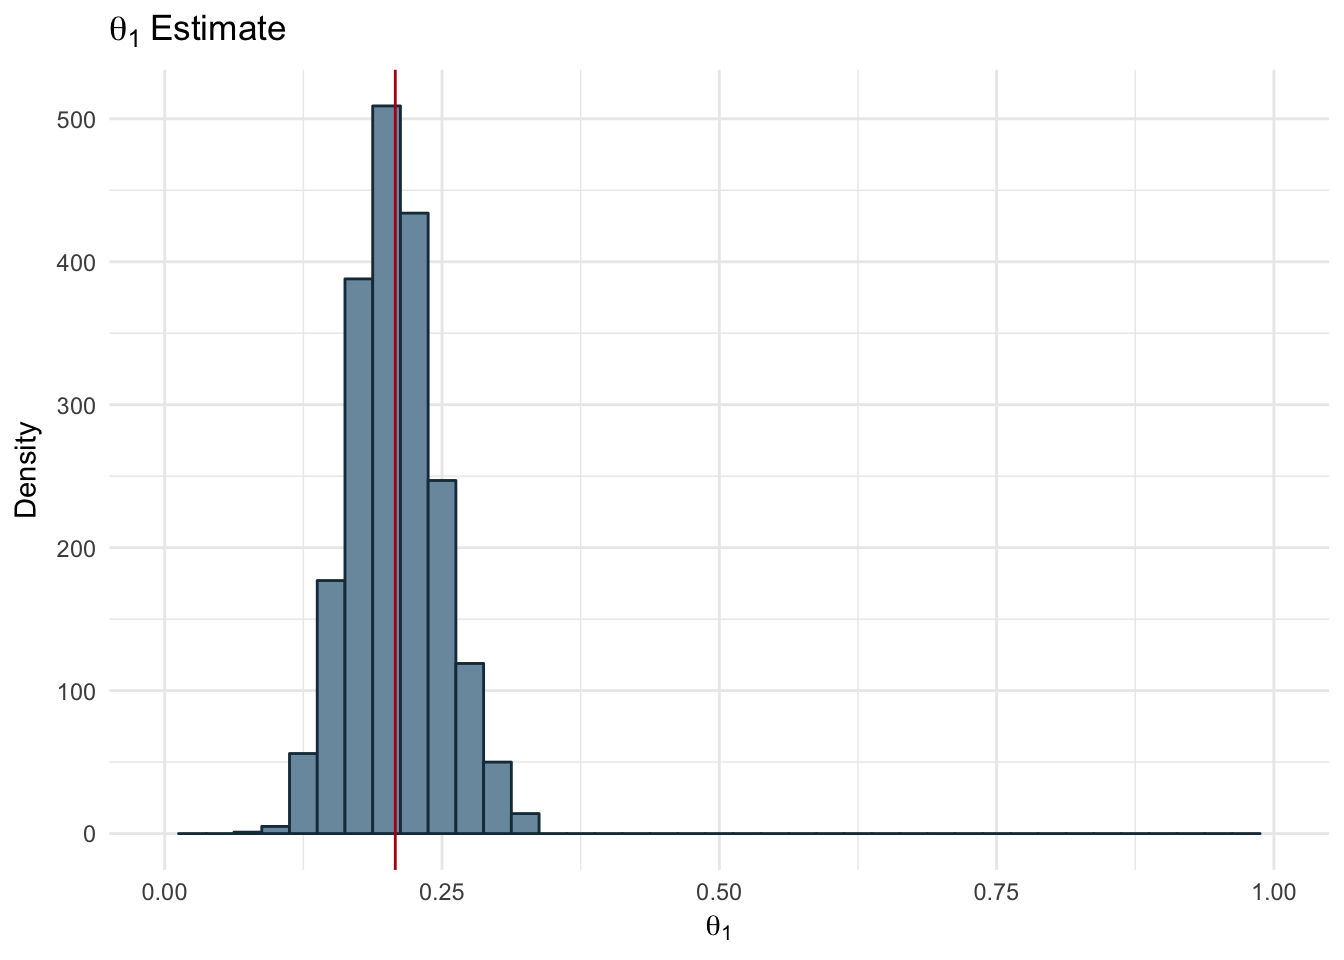
\includegraphics{_main_files/figure-latex/bernChangePointTheta1-1.pdf}
\caption{\label{fig:bernChangePointTheta1}Estimated Theta 1}
\end{figure}

\begin{Shaded}
\begin{Highlighting}[]
\KeywordTok{ggplot}\NormalTok{(params_df, }\KeywordTok{aes}\NormalTok{(}\DataTypeTok{x =}\NormalTok{ theta2)) }\OperatorTok{+}\StringTok{ }
\StringTok{  }\KeywordTok{geom_histogram}\NormalTok{(}\DataTypeTok{fill=}\StringTok{"#7A99AC"}\NormalTok{, }\DataTypeTok{color =}\StringTok{'#1A384A'}\NormalTok{ ) }\OperatorTok{+}\StringTok{ }
\StringTok{  }\KeywordTok{theme_minimal}\NormalTok{() }\OperatorTok{+}\StringTok{ }
\StringTok{  }\KeywordTok{geom_vline}\NormalTok{(}\DataTypeTok{xintercept =} \KeywordTok{mean}\NormalTok{(params_df}\OperatorTok{$}\NormalTok{theta2), }\DataTypeTok{color=}\StringTok{'#b7091a'}\NormalTok{) }\OperatorTok{+}
\StringTok{  }\KeywordTok{labs}\NormalTok{(}\DataTypeTok{title =} \KeywordTok{expression}\NormalTok{(theta[}\DecValTok{2}\NormalTok{]}\OperatorTok{~}\NormalTok{Estimate), }\DataTypeTok{x=}\KeywordTok{expression}\NormalTok{(theta[}\DecValTok{2}\NormalTok{]), }\DataTypeTok{y =} \StringTok{'Density'}\NormalTok{) }
\end{Highlighting}
\end{Shaded}

\begin{figure}
\centering
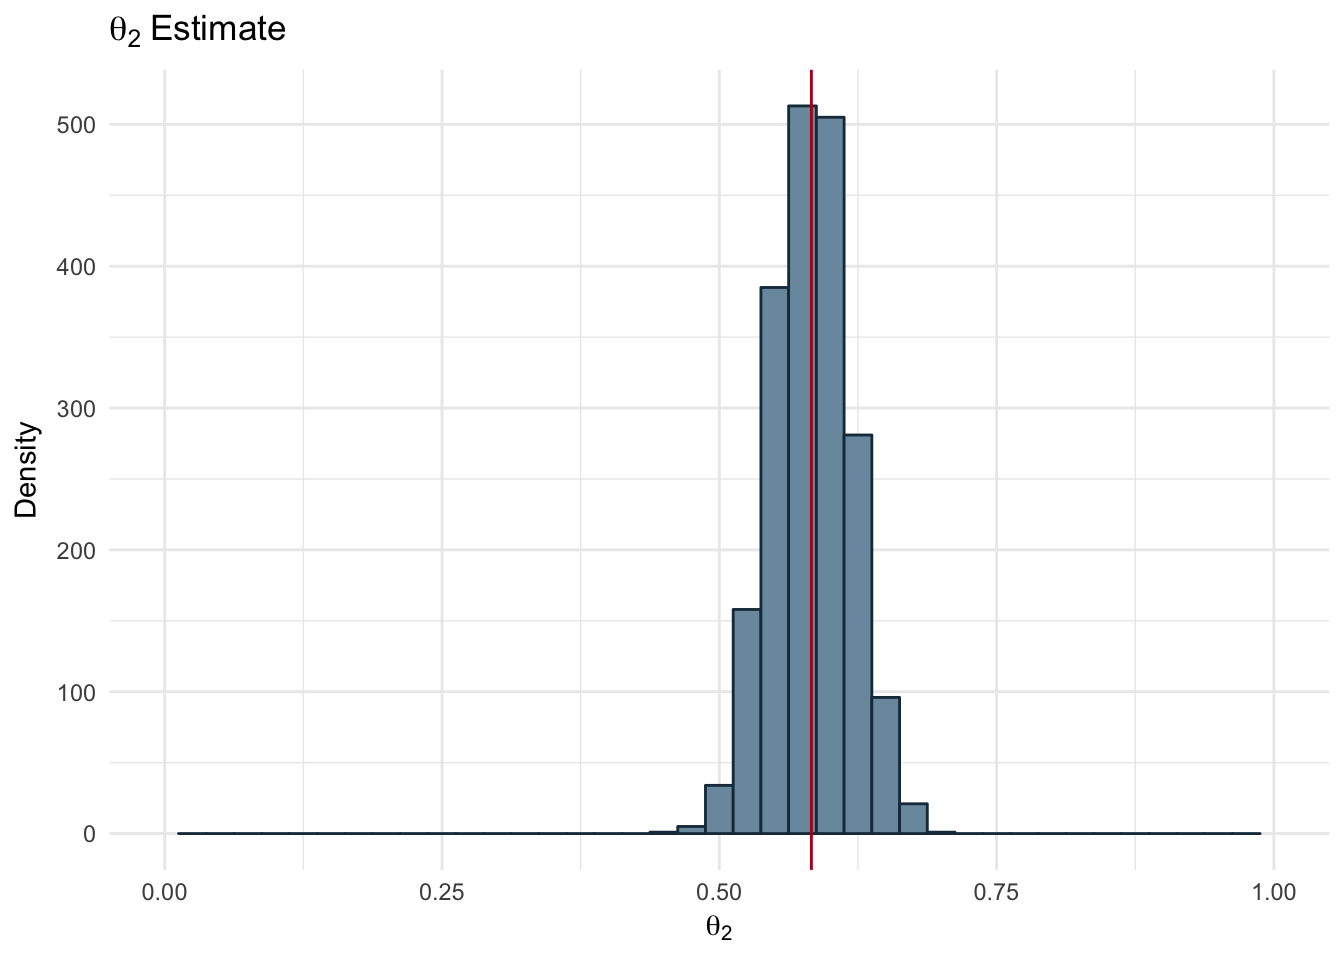
\includegraphics{_main_files/figure-latex/bernChangePointTheta2-1.pdf}
\caption{\label{fig:bernChangePointTheta2}Estimated Theta 2}
\end{figure}

\section{Summary}\label{summary}

\begin{itemize}
\tightlist
\item
  ML
\item
  MAP
\item
  Bayesian Inference
\item
  Gibbs Sampling
\item
  Evidence Term
\end{itemize}

\chapter{Multinomial Distribution}\label{multinomial-distribution}

\section{Comparison of Dice
vs.~Words}\label{comparison-of-dice-vs.words}

\section{Relationship to Bernoulli}\label{relationship-to-bernoulli}

\section{Conjugate Prior: Dirichlet}\label{conjugate-prior-dirichlet}

\section{Gibbs Sampling - Multinomial \&
Dirichlet}\label{gibbs-sampling---multinomial-dirichlet}

\subsection{Derivation of Gibbs Sampling Solution of Word Distribution
(Single
Doc)}\label{derivation-of-gibbs-sampling-solution-of-word-distribution-single-doc}

\chapter{Word Embeddings and
Representations}\label{word-embeddings-and-representations}

\section{Bag of Words}\label{bag-of-words}

\section{Word Embeddings}\label{word-embeddings}

\chapter{LDA as a Generative Model}\label{lda-as-a-generative-model}

\section{General Terminology}\label{general-terminology}

\section{Generative Model}\label{generative-model}

\subsection{Generating Documents}\label{generating-documents}

\subsubsection{Topic Word Mixtures, Document Topic Mixtures, and
Document Length
Static}\label{topic-word-mixtures-document-topic-mixtures-and-document-length-static}

\subsubsection{Topic Word Mixtures \& Document Topic Mixtures Static,
Document Length
Varying}\label{topic-word-mixtures-document-topic-mixtures-static-document-length-varying}

\subsubsection{Topic Word Mixtures Static, Varying Document Topic
Distributions and Document
Length}\label{topic-word-mixtures-static-varying-document-topic-distributions-and-document-length}

\subsection{LDA Generative Model}\label{lda-generative-model}

\chapter{LDA Inference}\label{lda-inference}

\section{General Overview}\label{general-overview}

Inference

\chapter{Placeholder}\label{placeholder}

\hypertarget{refs}{}
\hypertarget{ref-kerns2010introduction}{}
Kerns, G. 2010. \emph{Introduction to Probability and Statistics Using
R}. S.l: s.n.

\hypertarget{ref-Robinson2014beta}{}
Robinson, David. 2014. ``Understanding the Beta Distribution (Using
Baseball Statistics).''
\url{http://varianceexplained.org/statistics/beta_distribution_and_baseball/}.


\end{document}
